\documentclass{report}

\usepackage{color}
\usepackage{graphicx}
\usepackage{booktabs}
\usepackage{longtable}
\usepackage{amsmath}
\usepackage{amssymb}
\usepackage{bm}% bold math
\usepackage{slashed}
\usepackage{hyperref}
\usepackage[usenames,dvipsnames]{xcolor}
\usepackage[normalem]{ulem}

\def\invfb   {\ensuremath{\mbox{\,fb}^{-1}}\xspace}
\newcommand{\mev}{\ensuremath{\mathrm{\,Me\kern -0.1em V}}\xspace}
\newcommand{\mevc}{\ensuremath{{\mathrm{\,Me\kern -0.1em V\!/}c}}\xspace}
\newcommand{\mevcc}{\ensuremath{{\mathrm{\,Me\kern -0.1em V\!/}c^2}}\xspace}
\newcommand{\gev}{\ensuremath{\mathrm{\,Ge\kern -0.1em V}}\xspace}
\newcommand{\gevc}{\ensuremath{{\mathrm{\,Ge\kern -0.1em V\!/}c}}\xspace}
\newcommand{\gevcnospace}{\ensuremath{{\mathrm{\,Ge\kern -0.1em V\!/}c}}}
\newcommand{\gevcc}{\ensuremath{{\mathrm{\,Ge\kern -0.1em V\!/}c^2}}\xspace}
\newcommand{\bea}{\begin{eqnarray}}
\newcommand{\eea}{\end{eqnarray}}

\def\beq{\begin{equation}}
\def\eeq{\end{equation}}
\def\bea{\begin{eqnarray}}
\def\eea{\end{eqnarray}}

\newcommand{\gsim}{ \mathop{}_{\textstyle \sim}^{\textstyle >} }
\newcommand{\lsim}{ \mathop{}_{\textstyle \sim}^{\textstyle <} }
\newcommand{\ev}{{\rm eV}}
\newcommand{\kms}{{\rm km/s}}
\newcommand{\kev}{{\rm keV}}
\newcommand{\Mev}{{\rm MeV}}

\def\missET {\slashed{E}_T}
\def \bm#1{\mbox{\boldmath$#1$\unboldmath}} 
\def \myeq#1{(\ref{#1})}


%colors
\newcommand{\htr}[1]{{\color{red}  #1}}
\newcommand{\htb}[1]{{\color{blue}  #1}}
\newcommand{\htg}[1]{{\color{green}  #1}}
\newcommand{\hto}[1]{{\color{orange}  #1}}
\newcommand{\htp}[1]{{\color{Purple}  #1}}
\newcommand{\htm}[1]{{\color{magenta}  #1}}
\newcommand{\htrd}[1]{\htr{\st{#1}}}
\newcommand{\htbd}[1]{\htb{\sout{#1}}}
\newcommand{\htpd}[1]{\htp{\st{#1}}}
\newcommand{\htod}[1]{\hto{\st{#1}}}
\newcommand{\htgd}[1]{\htg{\st{#1}}}

\begin{document}

color code:

\htg{Priscilla}, \hto{Bjoern}, \htr{Krisztian}, \htb{Kevin}, \htm{Deborah}
\newline
\newline
\hto{BP: Todo: All tables need to be abbreviated to a sensible number of sig. digits.}

\section{Scalar s-channel Mediator}
\label{sec:scalar}
 
\hto{One of the most simple UV complete extension of the effective field theory approach is the addition of a scalar mediator between DM and SM.}
\sout{A scalar particle mediator can be a very simple addition to the SM}.  {\sout If it is chosen} \hto{In case this mediator is as a gauge singlet} it can have tree-level interactions with a singlet DM particle that is either a Dirac or Majorana fermion, or DM that  is a scalar itself. The spin-$0$ mediator \sout{could  still be chosen as} \hto{can  either be} a real or complex scalar, which are distinguished by the fact that a complex scalar contains both scalar and pseudoscalar particles, whereas the real \sout{option contains} \hto{field can be} only a scalar field. We will consider two choices for DM simplified models: one where the interaction with the SM is mediated by the real scalar, and the second where we consider only a light pseudoscalar (assuming that the associated scalar is decoupled from the low-energy spectrum). 
 
Couplings to the SM fermions can be arranged by mixing with the SM Higgs.  Such models have intriguing connections with Higgs physics, and can be viewed as generalizations of the Higgs portal to DM. The most general scalar mediator models will \sout{of course} have renormalizable interactions between the SM Higgs and the new scalar $\phi$ or pseudoscalar $a$, as well as $\phi/a$ interactions with electroweak gauge bosons. Such interactions are model dependent, often subject to constraints from electroweak precision tests, and would suggest specialized searches which cannot be generalized to a broad class of models (unlike, for instance, the \hto{$\missET+\textrm{jets}$} searches). As a result, for this class of \hto{minimal} simplified models with spin-$0$ mediators, we \sout{suggest to} \hto{will} focus primarily on \sout{the} couplings to fermions and \sout{the} loop-induced couplings to gluons. \sout{The possibility that the couplings} Possible couplings to the electroweak sector \hto{may} also lead to interesting DM phenomenology \sout{should however be kept in mind} \hto{BP: Broken sentence} and can be studied in the context of Higgs \hto{P}ortal DM.

\subsection{Fermionic DM}

Minimal Flavor Violation (MFV) \sout{dictates} \hto{implies} \sout{that the coupling of a scalar to the SM fermions} \hto{scalar couplings to fermions are} \sout{will be} proportional to the fermion mass\sout{es}.  However, \sout{it allows these couplings to be scaled by separate factors} \hto{can differ} for \sout{the up-type quarks, down-type quarks, and the} \hto{for up- and down-type quarks and} charged leptons. Assuming that DM is a fermion $\chi$, which couples to the SM only through a scalar $\phi$ or pseudoscalar $a$, the most general tree-level Lagrangians compatible with the MFV assumption are~\cite{Cotta:2013jna,Abdullah:2014lla}:
 \begin{eqnarray}
{\cal L}_{{\rm fermion},\phi} & = & {\cal L}_{\rm SM}+i\bar{\chi} \slashed{\partial} \chi + m_\chi \bar{\chi}\chi + \left| \partial_\mu \phi \right|^2+\frac{1}{2}m_\phi^2 \phi^2 + \nonumber \\ 
& &  g_\chi \phi \bar{\chi}\chi+ \frac{\phi}{\sqrt{2}} \sum_i \left(g_u y_i^u \bar{u}_i u_i+g_d y_i^d \bar{d}_i d_i+g_\ell y_i^\ell \bar{\ell}_i \ell_i\right)\, , \label{eq:scalarlag} \\
{\cal L}_{{\rm fermion},a} & = & {\cal L}_{\rm SM}+i\bar{\chi} \slashed{\partial} \chi + m_\chi \bar{\chi}\chi + \left| \partial_\mu a \right|^2+\frac{1}{2}m_a^2 a^2 + \nonumber \\
& &  ig_\chi a \bar{\chi}\gamma_5\chi+ \frac{i a}{\sqrt{2}}\sum_i  \left(g_u y_i^u \bar{u}_i \gamma_5 u_i+g_d y_i^d \bar{d}_i \gamma_5 d_i+g_\ell y_i^\ell   \bar{\ell}_i \gamma_5 \ell_i\right) \,. \label{eq:pseudoscalarlag}
\end{eqnarray}
Here the sums run over the \sout{there} \hto{all} SM \sout{families} \hto{generations} \sout{and we are using} \hto{the} Yukawa couplings $y_i^f$ \hto{are} normalized to $y_i^f = \sqrt{2}m_i^f/v$ \sout{with} \hto{where} $v \simeq 246 \, {\rm GeV}$ \hto{represents} the Higgs vacuum expectation value (VEV). \sout{Since the DM particle $\chi$ receives most of its mass most likely not from electroweak symmetry breaking but from another (unknown) mechanism, we parametrize the DM-mediator coupling by $g_\chi$ rather than by a Yukawa coupling $y_\chi = \sqrt{2}m_\chi/v$.}

\hto{BP: Previous sentence sounds speculating and I'd remove that, at least backup with reference. Prefer to just say: We parametrise the DM-mediator coupling as $g_\chi$.}

The most general Lagrangians including new scalars or pseudoscalars will have a potential  containing interactions with the SM Higgs field $h$. As \hto{already} stated \sout{above,} we choose \sout{to take a more} a minimal set of \sout{possible} interactions and leave the discussions of the couplings in the Higgs sector to \sout{the} section \sout{on} \hto{about}  Higgs portal DM. Given this simplification, the minimal set of parameters under consideration is
 \bea
  \left\{ m_\chi,~ m_{\phi/a},~ g_\chi,~ g_u,~ g_d,~ g_\ell \right\} \,.
 \eea
The simplest choice of couplings  \hto{known as Minimal Simplified Dark Matter model (MSDM) (following here notation used Buchm\"uller et al., Buckley et al. etc. which makes a lot of sense)}  $g_u = g_d = g_\ell$, which is realized in singlet scalar extensions of the SM. 

If one extends the SM Higgs sector to a two Higgs doublet model, one \sout{can} obtain\hto{s} \sout{other coupling patterns} \hto{more complex couplings} such as  $g_u = \cot \beta$ and $g_d = g_e = \tan \beta$ \sout{with} \hto{where} $\tan \beta$ denoting the ratio of VEVs of the two Higgs doublets.  The case $g_u \neq  g_d \neq g_\ell$ requires \sout{more} additional scalars \sout{, whose masses could be rather heavy} \hto{with potentially large masses}. 

\sout{For simplicity, we will use}\hto{We assume} universal SM-mediator couplings $g_v = g_u = g_d = g_\ell$ in the remainder of this work \sout{, though one should bear in mind that finding ways to experimentally  test this assumption would be very useful.} \hto{BP: That sounds like we don't know what we are doing. If there is no indication otherwise the easiest assumptions is always the most scientific to chose (also listening to some phenomenologists this seems not always to be the case ;-) )  }
 
The \sout{signal strength} \hto{The expected signal of DM pair production depends on the production rate defined by the dark matter mass $m_\chi$, mediator $m_{\phi/a}$ and the couplings $g_i$ and also the branching ration defined by the} total decay width of the mediator $\phi/a$. \sout{In the minimal model} \hto{While we cannot specify a width only from the couplings, we can calculate the minimum
possible width (assuming only decays into the dark matter and the Standard Model fermions) that is consistent with a given value of $g_\chi g_\textrm{SM}$. These are given by Eq.~\myeq{eq:width}}\cite{Buckley:2014fba}. 

\hto{BP: Removed the initial two equations as they are identical except of an index and used only one with proper indices and also two two line instead of extending beyond the text width.}


\begin{equation} \label{eq:width}
\begin{split}
\Gamma_{\phi,a}  = & \sum_f N_c \frac{y_f^2 g_v^2 m_{\phi,a}}{16 \pi} \left(1-\frac{4 m_f^2}{m_{\phi,a}^2}\right)^{3/2}
                   + \frac{g_\chi^2 m_{\phi,a}}{8 \pi} \left(1-\frac{4 m_\chi^2}{m_{\phi,a}^2}\right)^{3/2}\\
                 & + \frac{\alpha_s^2 y_t^2 g_v^2 m_{\phi,a}^3}{32 \pi^3 v^2} \left| f_{\phi,a}\left(\tfrac{4m_t^2}{m_{\phi,a}^2} \right)\right|^2
\end{split}
\end{equation}

%\begin{eqnarray}
%\Gamma_\phi & = & \sum_f N_c \frac{y_f^2 g_v^2 m_\phi}{16 \pi} \left(1-\frac{4 m_f^2}{m_\phi^2}\right)^{3/2} + \frac{g_\chi^2 m_\phi}{8 \pi} \left(1-\frac{4 m_\chi^2}{m_\phi^2}\right)^{3/2} + \frac{\alpha_s^2 y_t^2 g_v^2 m_\phi^3}{32 \pi^3 v^2} \left| f_\phi\left(\tfrac{4m_t^2}{m_\phi^2} \right)\right|^2 \,,  \label{eq:scalarwidth}  \hspace{8mm} \\
%\Gamma_a & = & \sum_f N_c \frac{y_f^2 g_v^2 m_a}{16 \pi} \left(1-\frac{4 m_f^2}{m_a^2}\right)^{1/2} + \frac{g_\chi^2 m_a}{8 \pi} \left(1-\frac{4 m_\chi^2}{m_a^2}\right)^{1/2}  
%+ \frac{\alpha_s^2 y_t^2 g_v^2 m_a^3}{32 \pi^3 v^2} \left| f_a\left(\tfrac{4m_t^2}{m_\phi^2} \right)\right|^2 \,, \label{eq:pseudoscalarwidth} 
%\end{eqnarray}


whereas

\bea \label{eq:fphifa}
f_\phi (\tau) = \tau \left [ 1+ (1-\tau) \arctan^2 \left ( \frac{1}{\sqrt{\tau-1}} \right ) \right ]  \,, \qquad 
f_a (\tau) =  \tau \arctan^2 \left ( \frac{1}{\sqrt{\tau-1}} \right ) \,. 
\eea

The first term in each width corresponds to the decay into SM fermions (the sum runs over all kinematically available fermions, $N_c = 3$ for quarks and $N_c = 1$ for leptons). The second term is the decay into DM (assuming that this decay is kinematically allowed). The factor of \sout{2} two between the decay into SM  fermions and into DM  is a result of our choice of normalization of the Yukawa couplings \hto{BP: Is this the best way to express that? I'd add:... due to spin dependencies}. The last two terms correspond to decay into gluons.  Since we have assumed that $g_v = g_u = g_d = g_\ell$, we have included in the partial decay widths $\Gamma (\phi/a \to gg)$ only the contributions stemming from top loops, which provide the by far largest corrections given that $y_t \gg y_b$~etc. At the loop level the mediators can decay not only to gluons but also to pairs of photons and other final states if \sout{these are} kinematical accessible. \hto{However} the decay rates $\Gamma (\phi/a \to gg)$ are \sout{however} always larger than the other loop-induced partial widths, and in consequence the total decay widths $\Gamma_{\phi/a}$ are well approximated by the corresponding sum of the individual partial decay widths involving DM, fermion or gluon pairs. \sout{Notice finally} \hto{It should be noted} that if  $m_{\phi/a} > 2m_t$ the total widths of $\phi/a$ will typically be dominated by the partial widths to top quarks.


%\section{DM production with $t\bar{t}$}
\section{DM+$t\bar{t}$ production}
\label{sec:ttdm}

\sout{As discussed in Section~\ref{sec:scalar}, the MFV assumption entails a spin-$0$ mediator that couples most strongly to top quarks on account of Yukawa couplings}.
\hto{As discussed in Sec.~\ref{sec:scalar}, the MFV assumption leads for spin-$0$ mediators to quark mass dependent Yukawa couplings and therefore dominant couplings to top quarks.}

\sout{ For establishing benchmarks, DM tt models with a scalar phi or a pseudoscalar a are the most compelling.}
\hto{[BP: Physics first:] Therefore DM+}$t\bar{t}$\hto{searches are strongly physically motivated and it is important to establish benchmarks for collider searches following the assumptions described in Sec.~\ref{sec:scalar}, in particular a Dirac fermion DM particle, universal couplings and minimum width.}
\sout{The simplifications mentioned in Section~\ref{sec:scalar} are followed; namely, coupling of the mediator to SM Higgs are not considered and universal SM-mediator couplings are assumed. Another simplification is to assume minimal width, so that }$\Gamma_{\phi,a}$\sout{is considered a dependent variable in the models. The DM particle is taken to be a Dirac fermion.}

\hto{Benchmark points have been selected to ensure that} \sout{The primary consideration for selecting the set of benchmark points is to ensure} the kinematic features of the parameter space are sufficiently represented. Detailed studies were performed to identify points in the $m_{\chi}$, $m_{\phi,a}$, $g_{\chi}$, $g_{v}$ (and $\Gamma_{\phi,a}$), parameter space that differ significantly from each other in terms of expected detector acceptance. Because missing \hto transverse momentum \sout{energy} is the key observable for searches, the mediator $p_{T}$ spectra is taken to represent the \hto{main} kinematics of a model. Another consideration in determining the set of benchmarks is to \sout{restrict to cases  where we have sensitivity} \hto{to focus on phase space where we expected to gain sensitivity during the LHC run in 2015}. Based on the \sout{estimated} \hto{projected} integrated luminosity of $30\,{\rm fb}^{-1}$ expected \hto{for} 2015, we disregard models \hto{with} cross section times branching ratio smaller than $0.1\,{\rm fb}$.

\subsection{Parameter scan}
The kinematics \sout{show the strongest dependence} \hto{is most dependent} on the masses $m_{\chi}$ and $m_{\phi,a}$. \hto{Figure~\ref{fig:scanPhi} and~\ref{fig:scanPhiPseudo} show typical depenencies
for for scalar, pseudoscalar couplings respectively.}
\sout{Examples of the dependence on mediator mass are given in Figs.\sout{ures}~\ref{fig:scanPhi} and~\ref{fig:scanPhiPseudo} for the scalar and pseudoscalar respectively}.\sout{ There are} \hto{The} two relevant thresholds \hto{are}: $m_{\phi,a} = 2m_{\chi}$ and $m_{\phi,a} = 2m_t$. When the mediator \hto{mass exceeds} both \sout{these} thresholds \hto{then} the $p_{T}$ spectra broadens with larger $m_{\phi,a}$ and the kinematics for $\phi$ and $a$ are \sout{quite similar} \sout{comparable}. The mediator $p_{T}$ spectra changes significantly when crossing these thresholds. \hto{For instance} \hto{In particular} kinematics are different for an on-shell mediator compared to an off-shell mediator ($m_{\phi,a}<2m_{\chi}$). Furthermore, the scalar \hto{case} differs from the pseudoscalar \hto{one} when $m_{\phi}<2m_t$. Therefore, it is important to \sout{have benchmark points } cover both sides of these thresholds \hto{with sufficient benchmark points}.

\begin{figure}[!ht]
  \begin{center}
    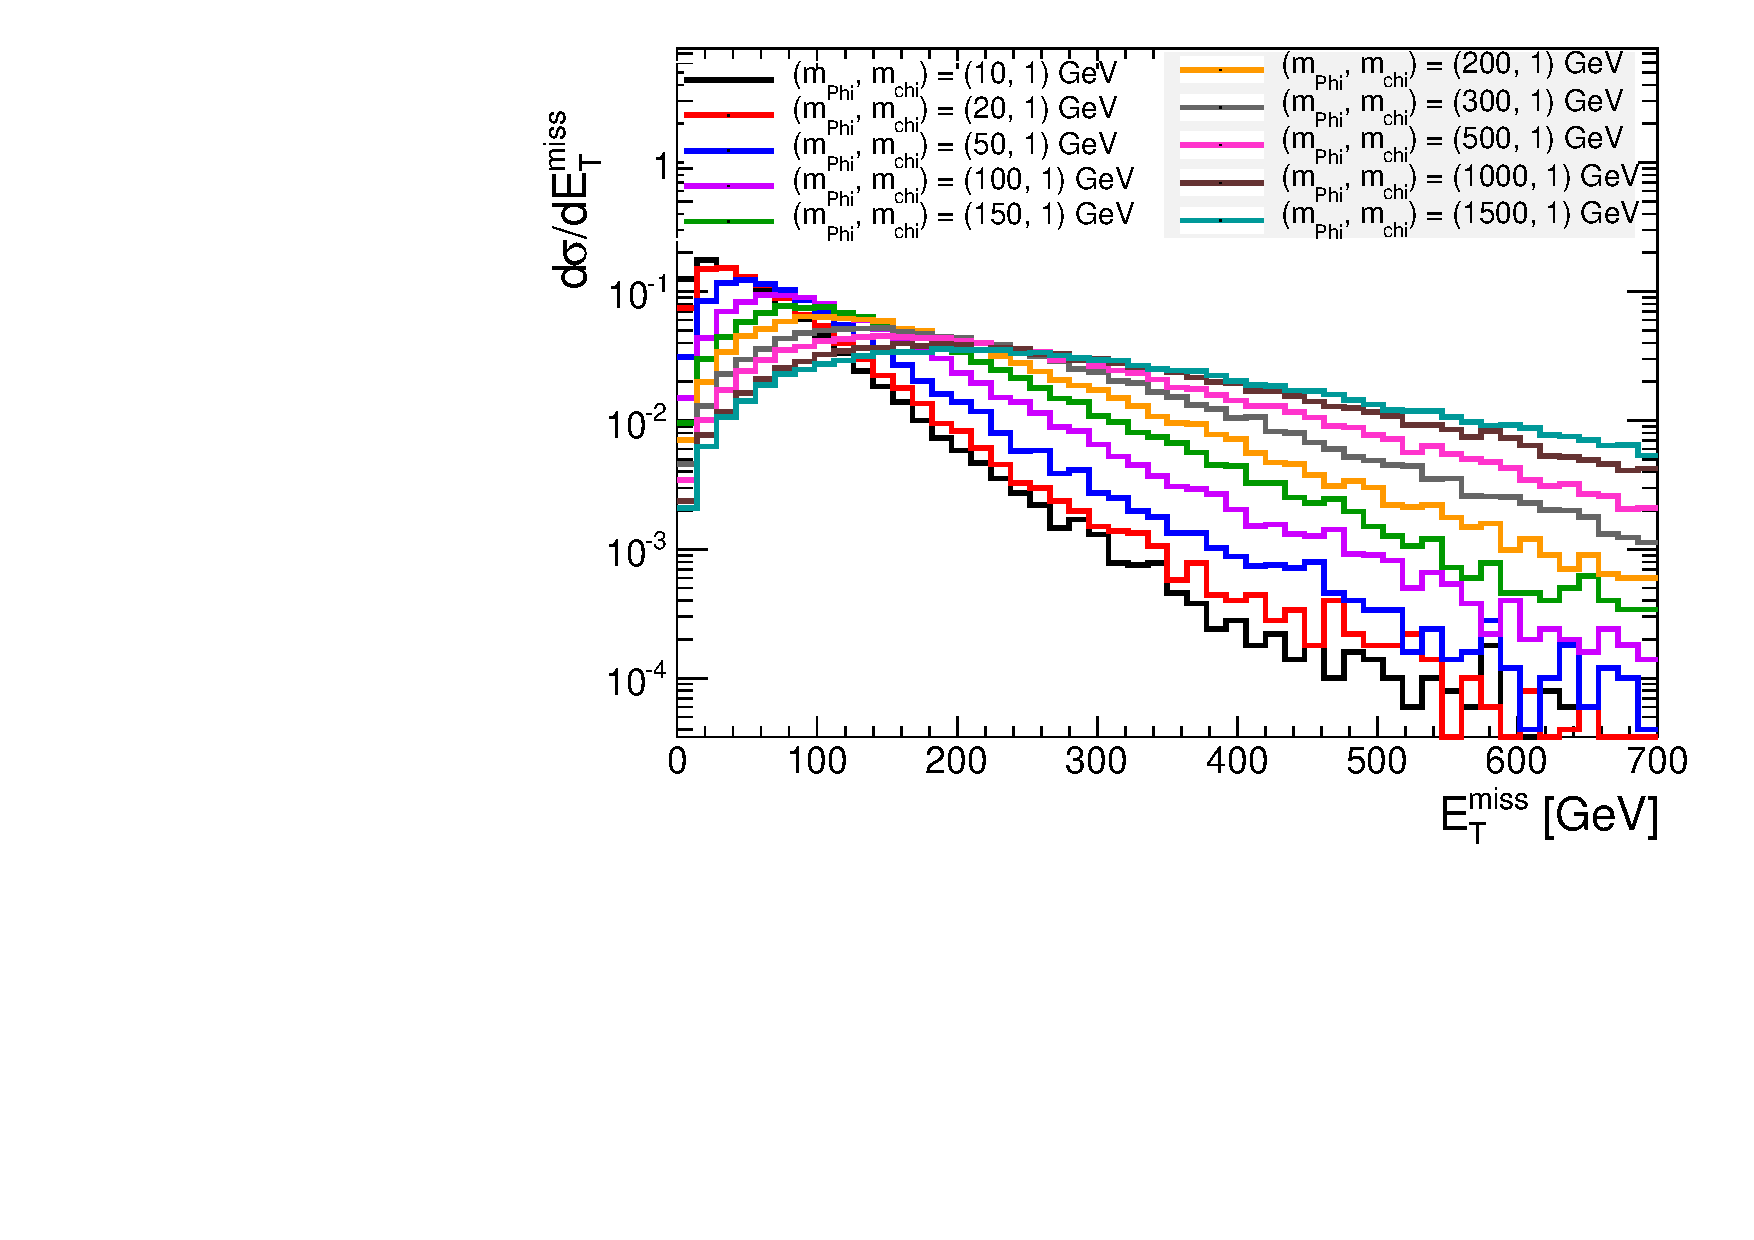
\includegraphics[scale=0.45]{figures/MEt_chi1.pdf}
    \vspace{2mm}
    \caption{\label{fig:scanPhi} \htg{Example of the dependence of the kinematics on the scalar mediator mass. The Dark Matter mass is fixed to be $1 {\rm GeV}$.}
    }
\end{center}
\end{figure}


\begin{figure}[!ht]
  \begin{center}
    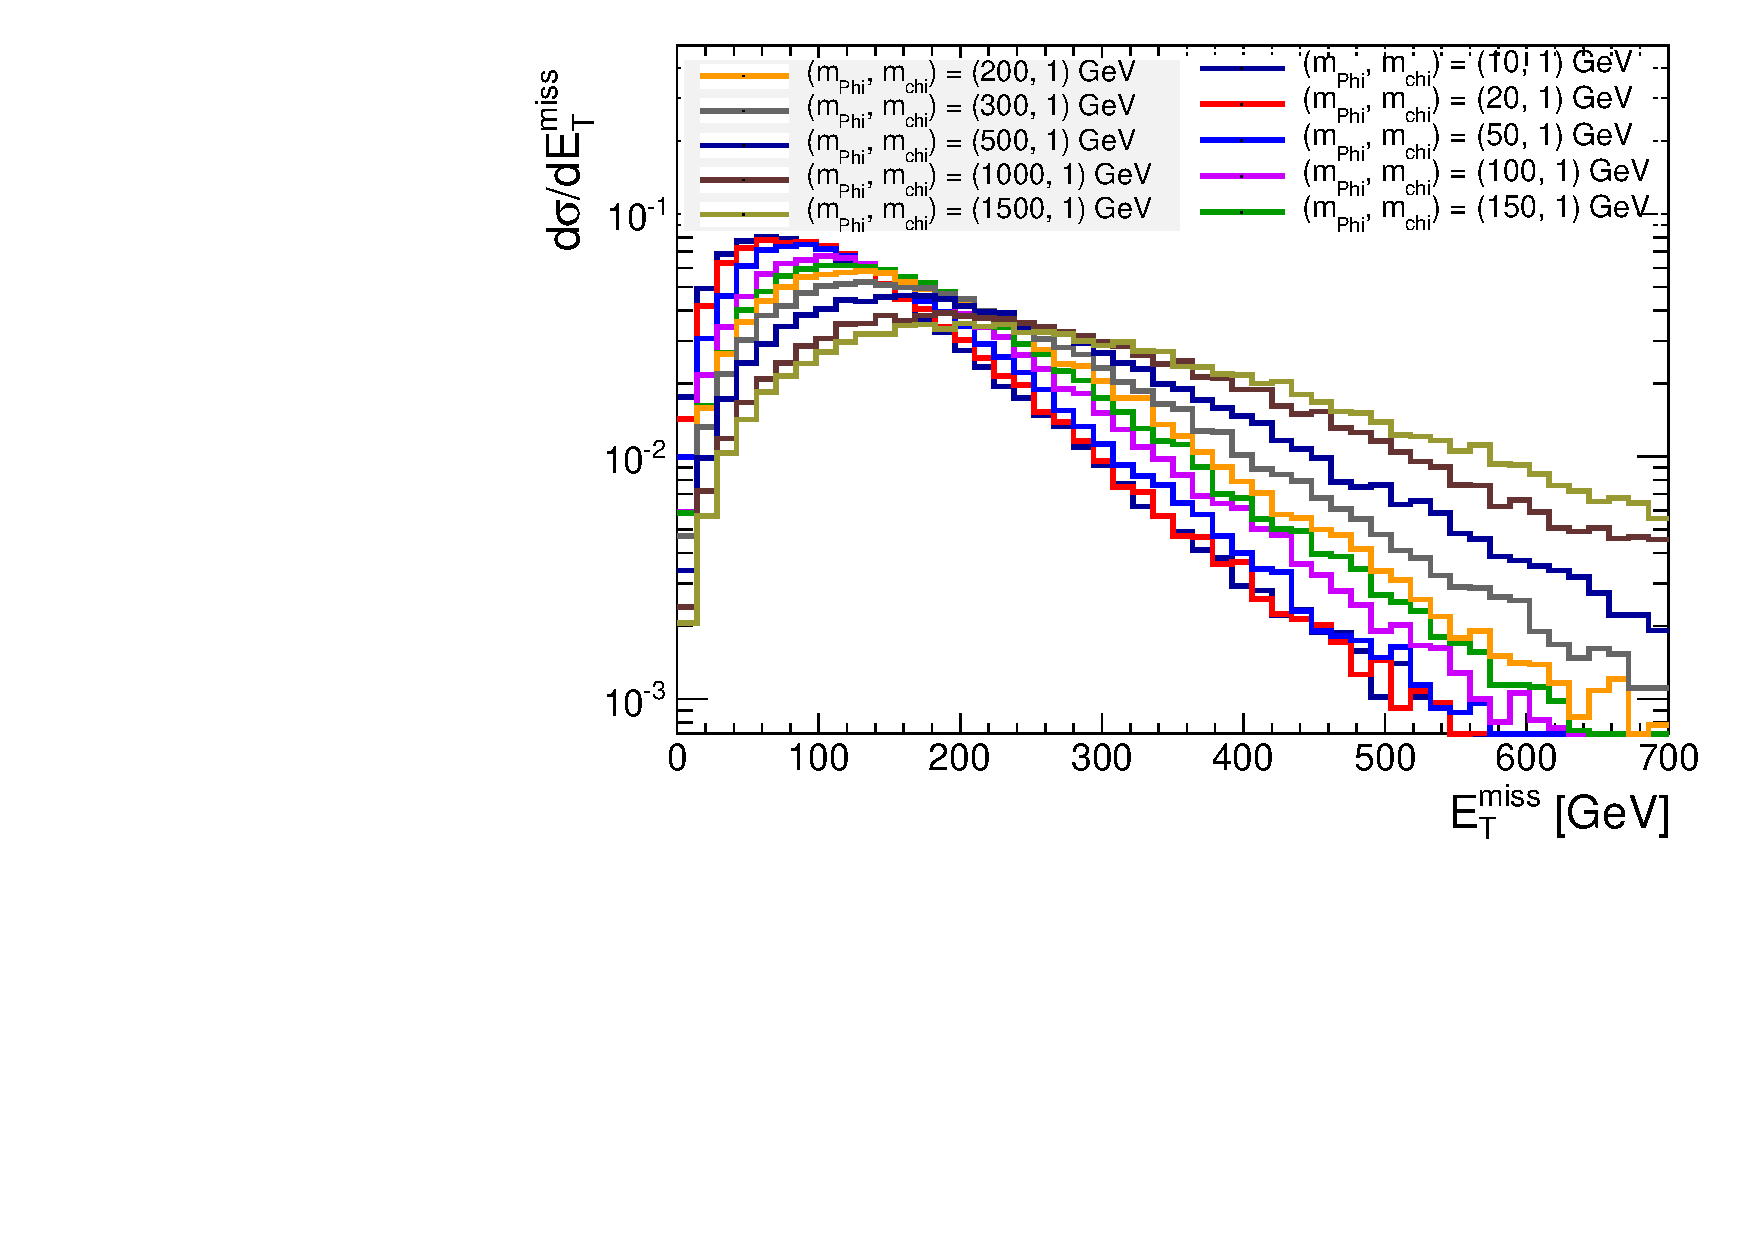
\includegraphics[scale=0.45]{figures/MEt_chi1_pseudo.pdf}
    \vspace{2mm}
    \caption{\label{fig:scanPhiPseudo} \htg{Example of the dependence of the kinematics on the pseudoscalar mediator mass. The Dark Matter mass is fixed to be $1 {\rm GeV}$.}
    }
\end{center}
\end{figure}

\begin{figure}[!ht]
  \begin{center}
    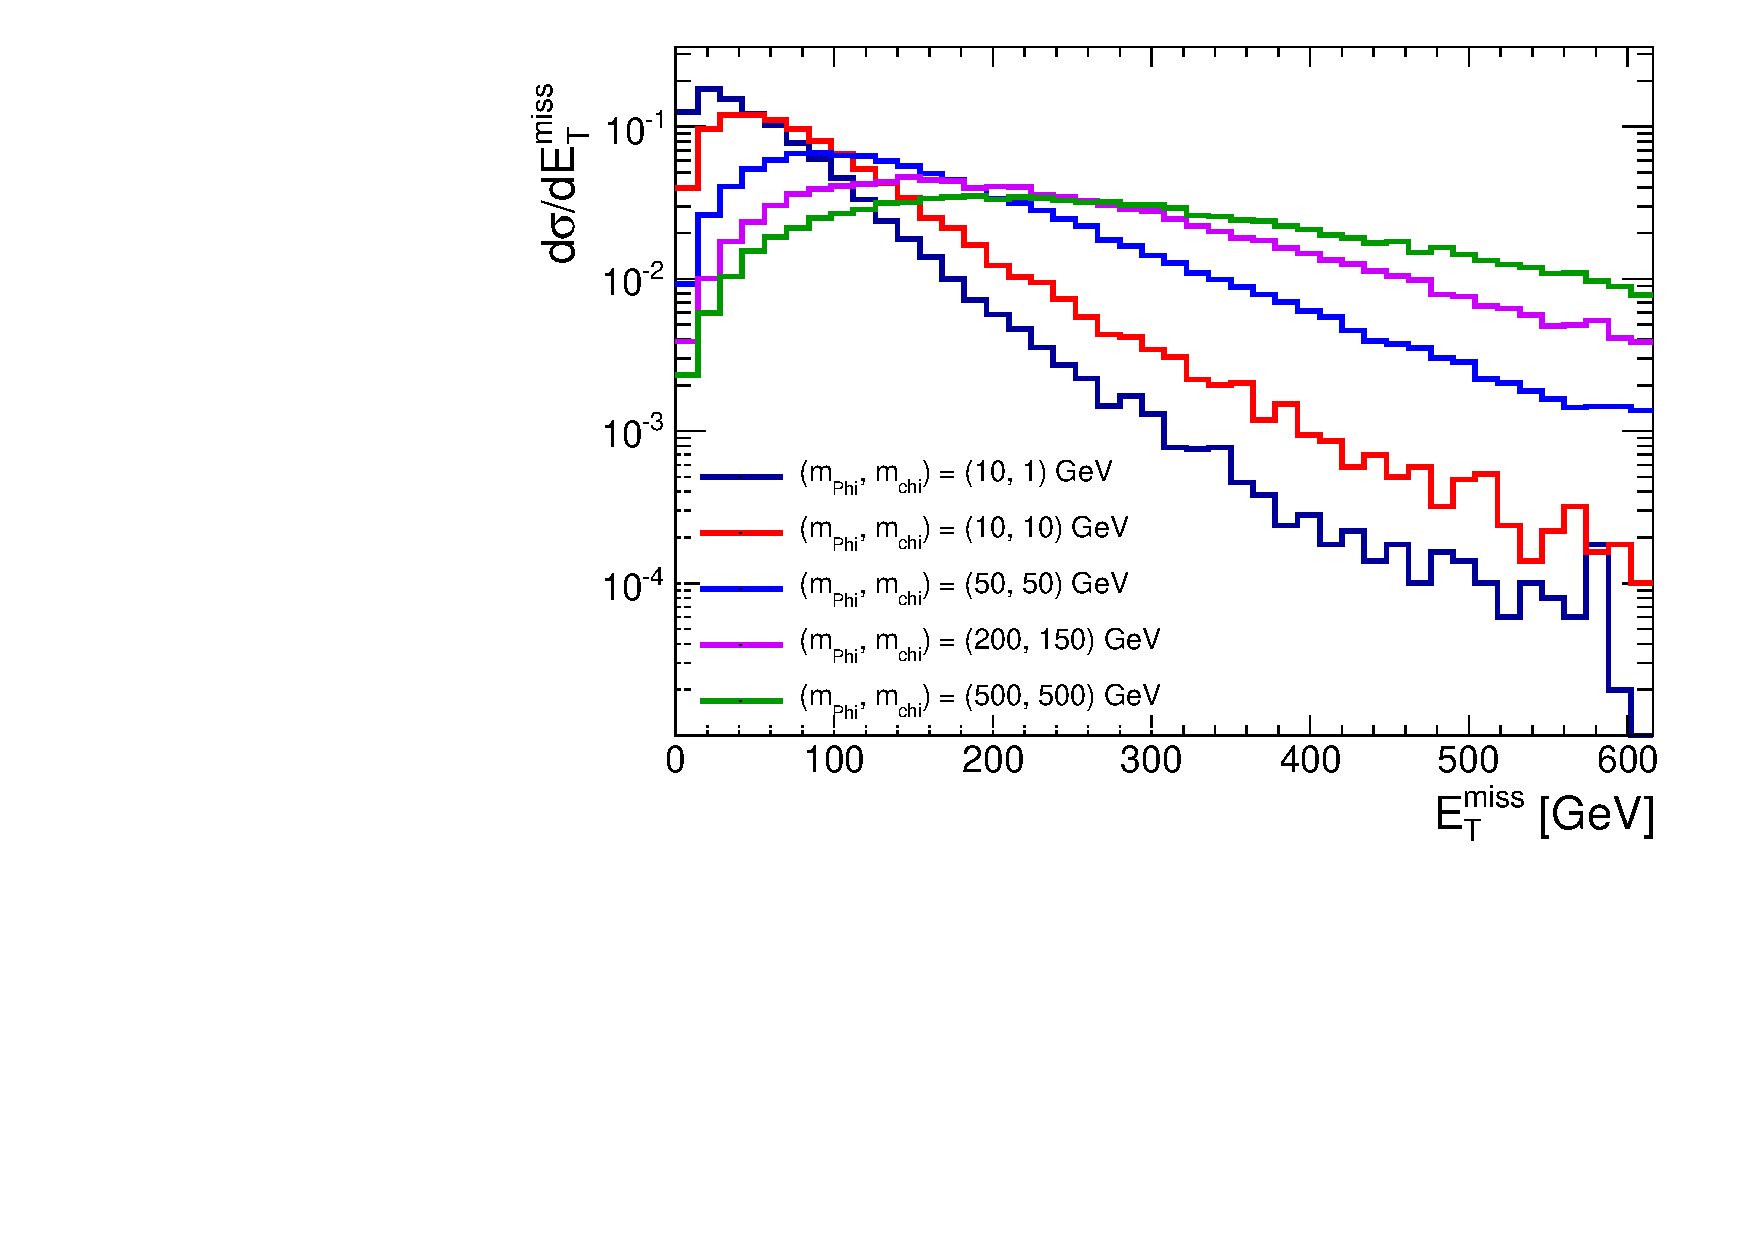
\includegraphics[scale=0.45]{figures/MEt_diagonal_scan.pdf}
    \vspace{2mm}
    \caption{\label{fig:scanPhidiag} \htg{Example of the dependence of the kinematic for points of the grid proposed in Tab.~\ref{tab:ttdm_benchmarks} close to the $m_{\phi,a} \sim 2m_\chi$ limit.}
    }
\end{center}
\end{figure}


%{\color{red} Add plot: $m_{\chi}$ scan}
%{\color{red} Add plot: on-shell vs off-shell}
%{\color{red} Add plot: S vs PS for $m_{\phi} < 2m_t$}

Typically, \sout{the kinematics show little dependence on the width -- or equivalently on the couplings} \hto{typically only weak dependencies on width or equivalently couplings are observed}  (see Fig.\sout{ure}~\ref{fig:widthsmallscan}), except \sout{at} \hto{for} large mediator masses of $\sim 1.5\,{\rm TeV}$ or \hto{for} very small couplings of $\sim 10^{-2}$. These regimes where width effects are significant have \sout{signal strengths} \hto{production cross section} that are too \sout{weak} \hto{small} to be relevant for $30\,{\rm fb}^{-1}$ and are not considered here. However, with the full dataset of Run-2, such models may be within reach. The generally weak dependence on typical width values can be understood as the parton distribution function \sout{being} \hto{are} the dominant effect on mediator production. In other words, for couplings $\sim O(1)$ the width is \sout{broad} \hto{large} enough that the $p_T$ of the mediator is determined mainly by the PDF.

\begin{figure}[!ht]
  \begin{center}
    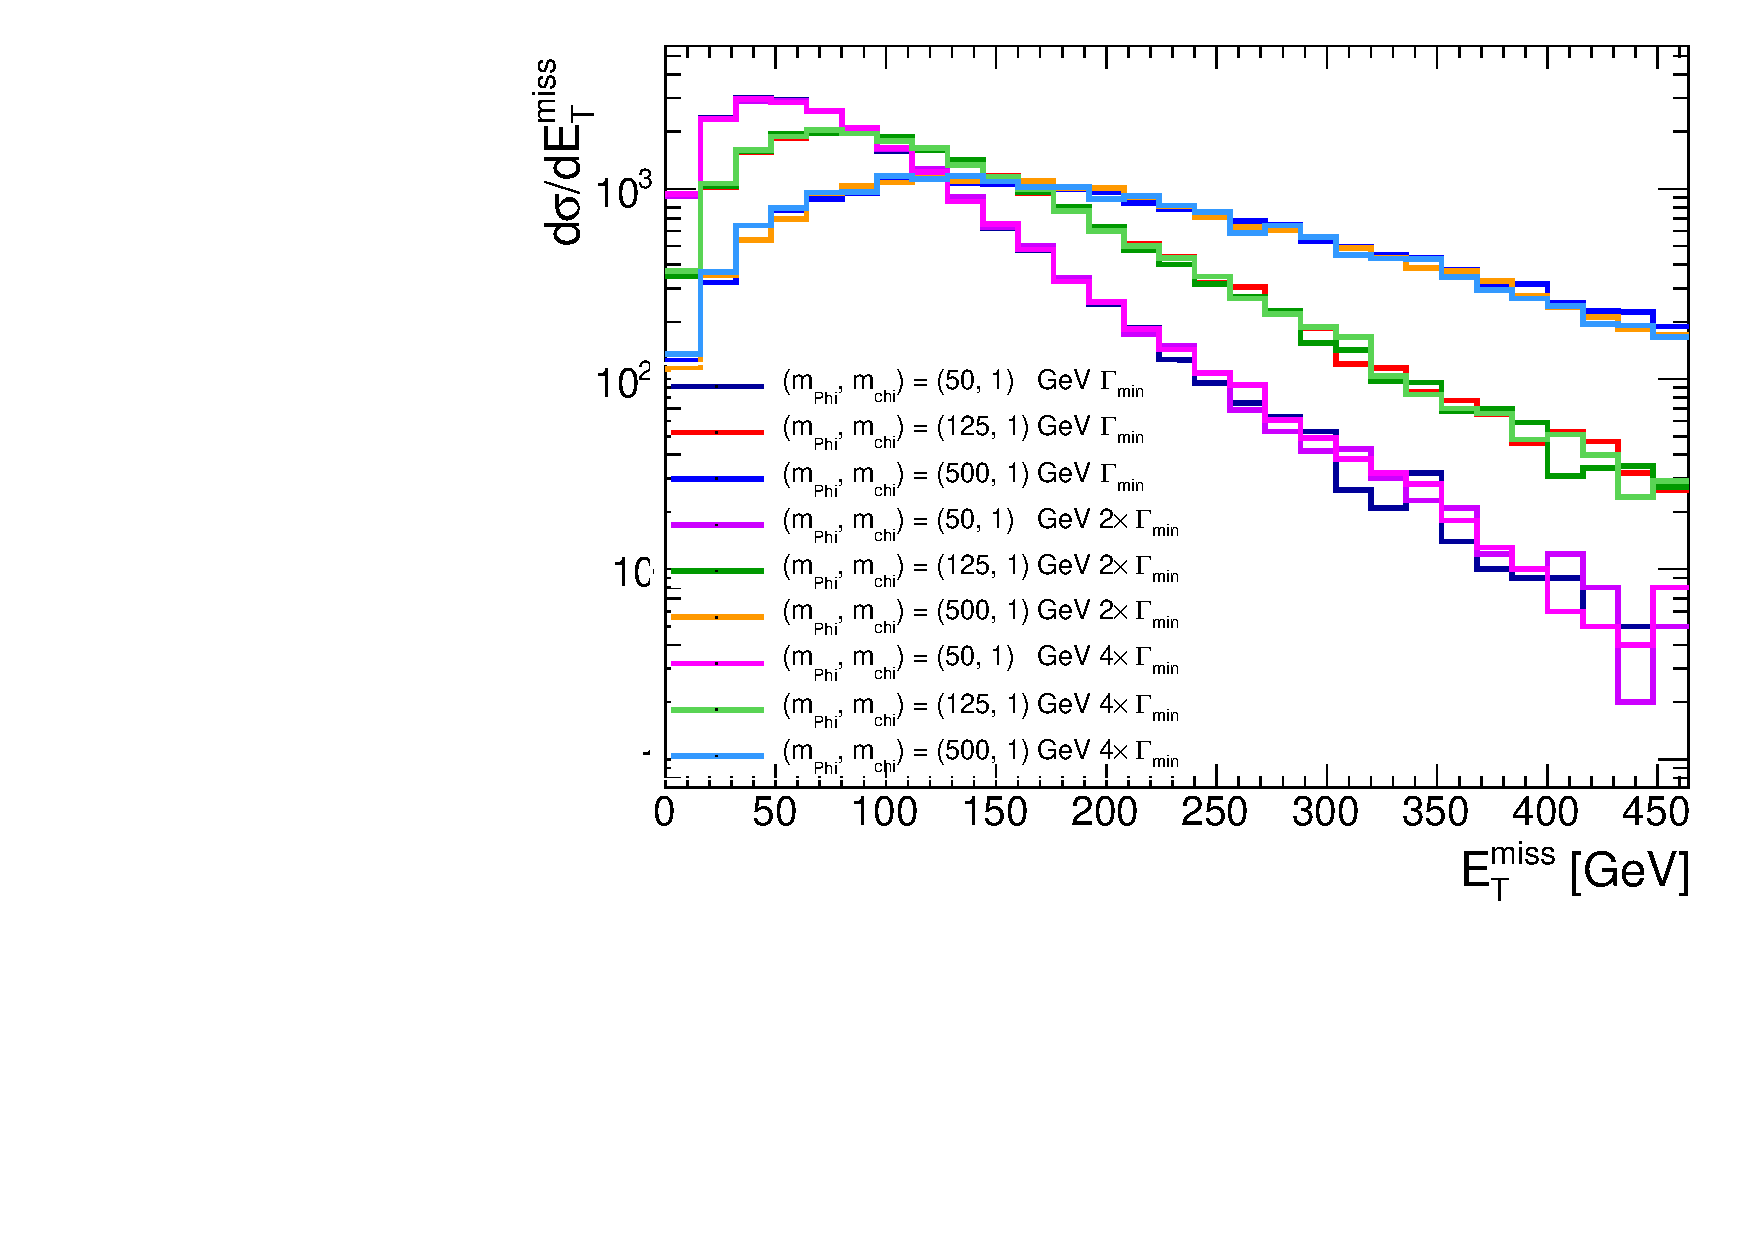
\includegraphics[scale=0.45]{figures/MEt_smallwidth.pdf}
    \vspace{2mm}
    \caption{\label{fig:widthsmallscan} \htg{Study of the dependence of kinematics on the width of a scalar mediator. The width is increased up to four times the minimal width for each mediator and dark matter mass combination. }
    }
\end{center}
\end{figure}

Another case where the width can impact the kinematics is when $m_{\phi,a}$ is slightly larger than $2m_\chi$. Here, the width determines the relative contribution between on-shell and off-shell production. An example is given in Fig.\sout{ure}~\ref{fig:widthlargescan}. \htg{In our reccomendations we propose to use for semplicity the minimal width, as this is represents the most conservative choice to interpret the LHC results}

\begin{figure}[!ht]
  \begin{center}
    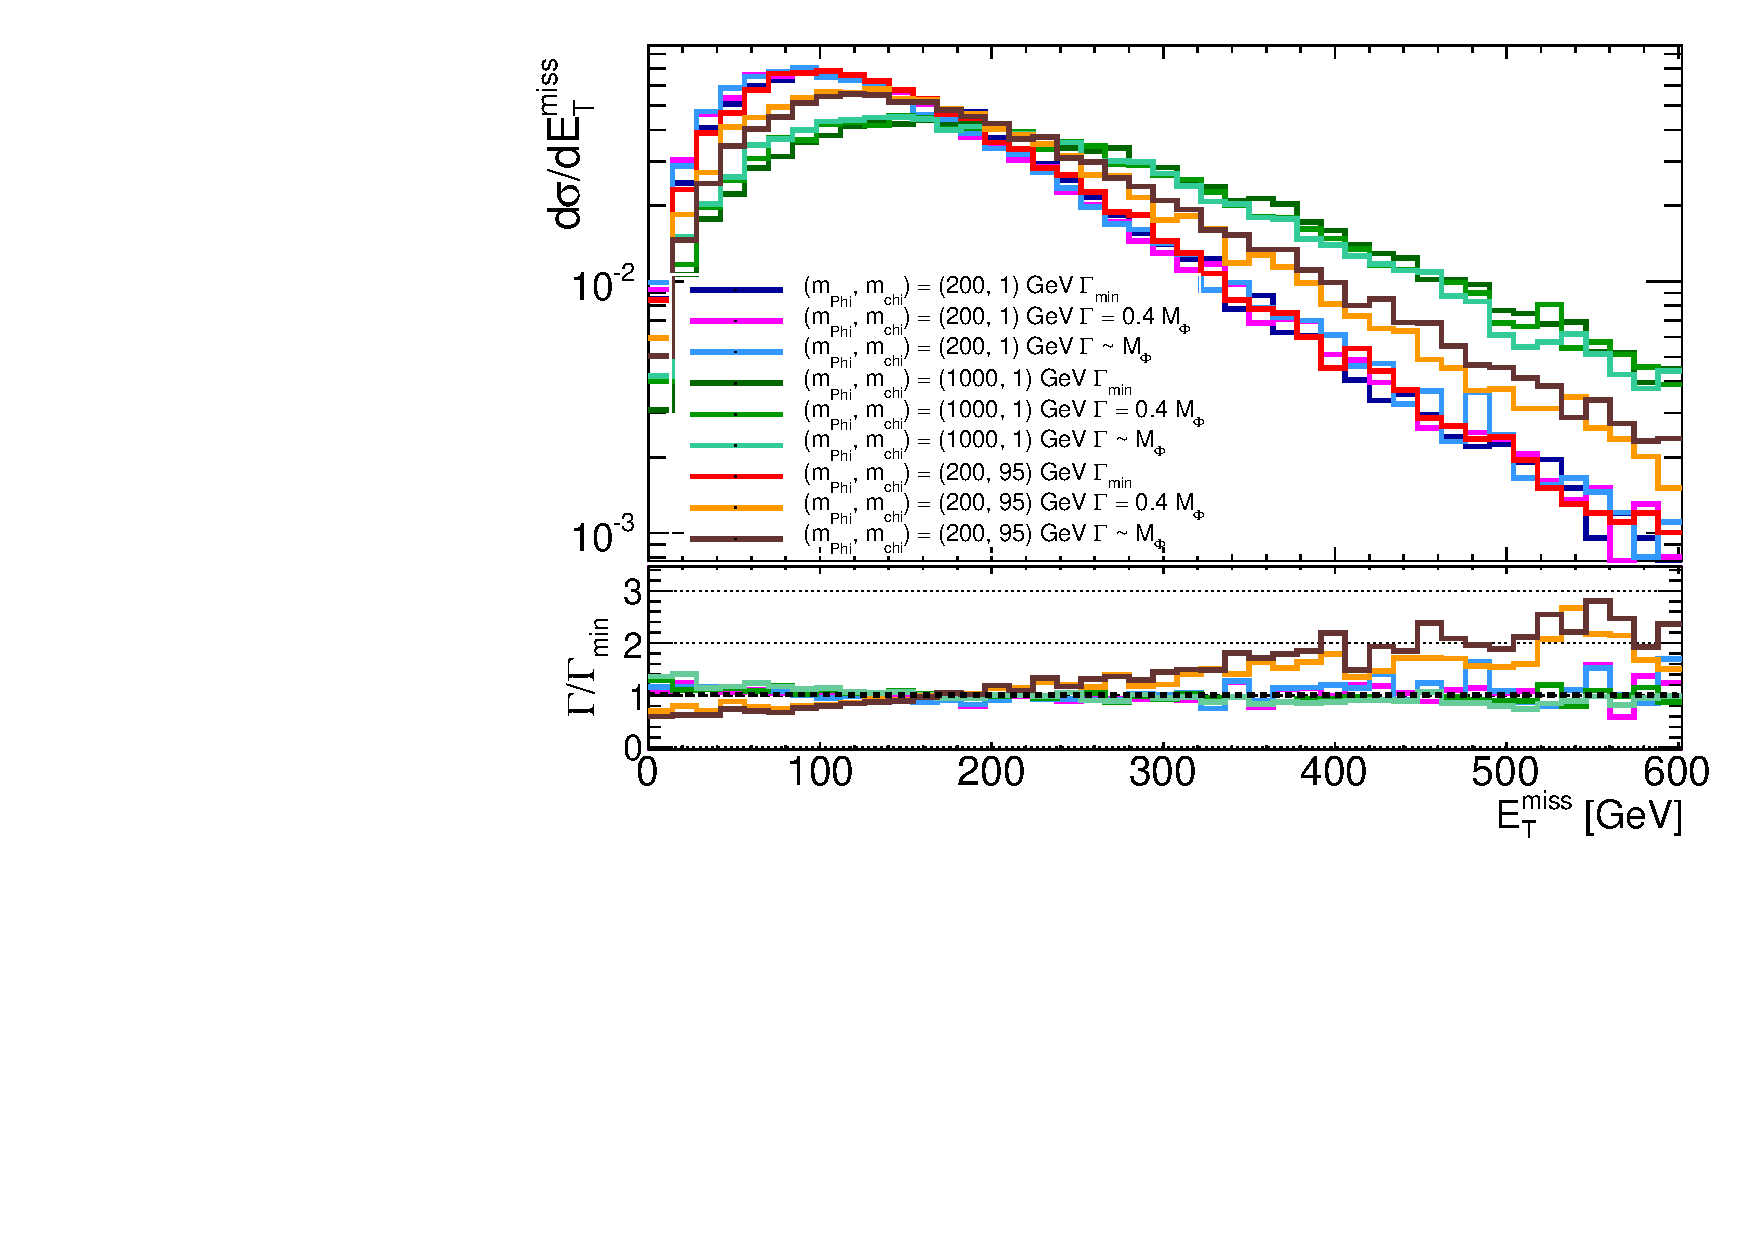
\includegraphics[scale=0.45]{figures/ScalarWidth.pdf}
    \vspace{2mm}
    \caption{\label{fig:widthlargescan} \htg{Dependence of the dependence of kinematics on the width of a scalar mediator. The width is increased up to the mediator mass. Choices of mediator and dark matter masses such that $m_{\phi,a}$ is slightly larger than $2m_\chi$ is the only case that shows a sizeable variation of the kinematics as a function of the width.  }
    }
\end{center}
\end{figure}

%{\color{red} Add plot: scan of couplings at $m_{\phi}=1.5\,{\rm TeV}$ to show kinematic differences}

Given that the kinematics are similar for all couplings $\sim O(1)$, we \sout{make a simplification to generate benchmark models with} \hto{we generate only samples with} $g_{\chi} = g_{v} = 1$. It follows that the model should be a good approximation for non-unity couplings and $g_{\chi} \neq g_{v}$ provided that the sample is normalized to the appropriate cross section times branching ratio. While a simple scaling function can be found that works for a limited range of coupling values (see Fig.\sout{ure}~\ref{fig:xsec_scaling} for example), we \sout{opt} \hto{chose} to provide instead a table of cross section times branching ratio values over a large range of couplings to support interpretation of search results (see Sec.tion~\ref{subsec:xsectable}). The table \hto{covers} lists couplings from $g=0.1$ to $g=3.5$, where the upper limit is chosen to \sout{lie near but below the} \hto{close to the} perturbative limit.

\begin{figure}[!ht]
\begin{center}
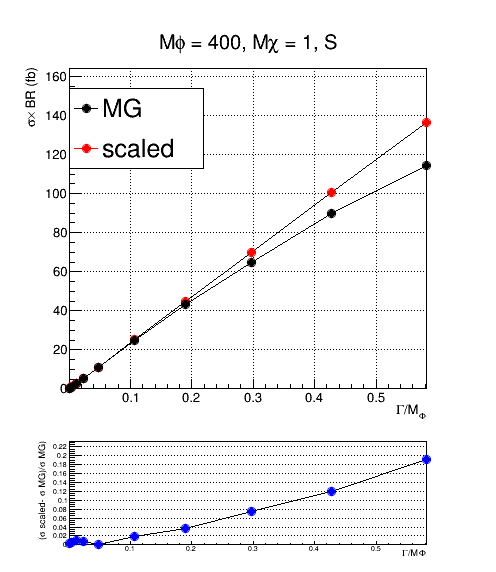
\includegraphics[scale=0.45]{figures/xVSwom_mphi_400_mchi_1_proc_S.png}
\vspace{2mm}
\caption{\label{fig:xsec_scaling} An example comparing a simple cross section scaling versus the computation from the generator, for a scalar model with $m_{\phi}=400\,{\rm GeV}$ and $m_{\chi}=1\,{\rm GeV}$. In this example, the scaling relationship holds for $\Gamma_{\phi}/m_{\phi}$ below $0.2$, beyond which finite width effects become important and the simple scaling breaks down.}
\end{center}
\end{figure}





\subsection{Benchmarks}
The benchmark points are listed in Table~\ref{tab:ttdm_benchmarks}. In addition to the considerations discussed in the preceding subsections, very light DM fermions are included ($m_{\chi}=1, 10\,{\rm GeV}$) as these are beyond the reach of current direct detection experiments, and a few points are chosen to overlap with monojet benchmarks to facilitate comparison with searches in different final states.


\begin{table}[!ht]
\centering
\begin{tabular}{| l | r |}
\hline
\multicolumn{1}{|c|}{$m_{\chi}$ (${\rm GeV}$)} & \multicolumn{1}{c|}{$m_{\phi,a}$ (${\rm GeV}$)} \\
\hline
 $1$    & $10$, $20$, $50$, $100$, $150$, $200$, $300$, $500$, $1000$, $1500$  \\
 $10$   & $10$, $20$, $50$, $100$, $150$, $200$, $300$, $500$, $1000$, $1500$  \\
 $50$   &             $50$, $100$, $150$, $200$, $300$, $500$, $1000$, $1500$  \\
 $150$  &                          $150$, $200$, $300$, $500$, $1000$, $1500$  \\
 $500$  &                                               $500$, $1000$, $1500$  \\
\hline
\end{tabular}
\caption{Simplified model benchmarks for $t\bar{t}$+DM production via spin-0 mediators decaying to Dirac DM fermions taking the minimum width presciption for $g_v = g_{\chi} = 1$.}
\label{tab:ttdm_benchmarks}
\end{table}

\newpage
\subsection{Table of Cross Sections}
\label{subsec:xsectable}
\begin{longtable}{lllll}
\toprule
Coupling (g) & $m_{Phi}$ [GeV] & $m_{\chi}$ [GeV] & $\Gamma_{min}$ [GeV] & $\sigma$\\
\midrule
\endfirsthead

\multicolumn{5}{c}{\tablename\ \thetable{} -- continued from previous page} \\
Coupling (g) & $m_{Phi}$ [GeV] & $m_{\chi}$ [GeV] & $\Gamma_{min}$ [GeV] & $\sigma$\\
\midrule
\endhead

\midrule
\multicolumn{5}{r}{{Continued on next page}} \\ 
\endfoot

\bottomrule
\endlastfoot

 0.1 &    10 &     1 & 0.00374318 &    0.207 $\pm$ 0.0006846 \\
 0.1 &    20 &     1 & 0.00784569 &   0.1121 $\pm$ 0.0003285 \\
 0.1 &    50 &     1 &  0.01987 &  0.03211 $\pm$ 0.0001005 \\
 0.1 &   100 &     1 & 0.0398141 & 0.007325 $\pm$ 2.416e-05 \\
 0.1 &   150 &     1 & 0.0597437 & 0.002396 $\pm$ 7.419e-06 \\
 0.1 &   200 &     1 & 0.0796724 & 0.001018 $\pm$ 3.398e-06 \\
 0.1 &   300 &     1 & 0.119549 & 0.0003394 $\pm$ 1.234e-06 \\
 0.1 &   500 &     1 & 0.310863 & 6.802e-05 $\pm$ 2.343e-07 \\
 0.1 &  1000 &     1 & 0.881329 & 5.817e-06 $\pm$ 2.356e-08 \\
 0.1 &  1500 &     1 &  1.40417 & 8.942e-07 $\pm$ 3.832e-09 \\
 0.1 &    10 &    10 & 0.000100 & 1.007e-05 $\pm$ 3.761e-08 \\
 0.1 &    20 &    10 & 0.000100  & 3.491e-05 $\pm$ 1.012e-07 \\
 0.1 &    50 &    10 & 0.0153395 &  0.03212 $\pm$ 0.0001037 \\
 0.1 &   100 &    10 & 0.0374747 & 0.007343 $\pm$ 2.011e-05 \\
 0.1 &   150 &    10 & 0.0581752 & 0.002389 $\pm$ 7.654e-06 \\
 0.1 &   200 &    10 & 0.0784937 & 0.001018 $\pm$ 6.258e-06 \\
 0.1 &   300 &    10 & 0.118762 & 0.0003373 $\pm$ 1.448e-06 \\
 0.1 &   500 &    10 & 0.310391 & 6.773e-05 $\pm$ 2.326e-07 \\
 0.1 &  1000 &    10 & 0.881093 & 5.81e-06 $\pm$ 2.245e-08 \\
 0.1 &  1500 &    10 &  1.40401 & 8.937e-07 $\pm$ 4.013e-09 \\
 0.1 &    50 &    50 & 0.0000233555 & 2.581e-07 $\pm$ 1.214e-09 \\
 0.1 &   100 &    50 & 0.0000492402 & 1.526e-06 $\pm$ 7.038e-09 \\
 0.1 &   150 &    50 & 0.0247905 & 0.002387 $\pm$ 8.272e-06 \\
 0.1 &   200 &    50 & 0.051794 &  0.00102 $\pm$ 3.216e-06 \\
 0.1 &   300 &    50 & 0.100226 & 0.0003366 $\pm$ 1.393e-06 \\
 0.1 &   500 &    50 & 0.299052 & 6.679e-05 $\pm$ 2.406e-07 \\
 0.1 &  1000 &    50 & 0.875378 & 5.764e-06 $\pm$ 2.472e-08 \\
 0.1 &  1500 &    50 &   1.4002 & 8.866e-07 $\pm$ 3.257e-09 \\
 0.1 &   100 &   150 & 0.0000492402 & 1.246e-08 $\pm$ 5.121e-11 \\
 0.1 &   150 &   150 & 0.0000765167 & 1.393e-08 $\pm$ 6.653e-11 \\
 0.1 &   200 &   150 & 0.000106902 & 1.693e-08 $\pm$ 8.493e-11 \\
 0.1 &   300 &   150 & 0.000190543 & 7.557e-08 $\pm$ 2.171e-10 \\
 0.1 &   500 &   150 & 0.213784 & 5.063e-05 $\pm$ 1.724e-07 \\
 0.1 &  1000 &   150 & 0.828844 & 5.365e-06 $\pm$ 2.028e-08 \\
 0.1 &  1500 &   150 &  1.36872 & 8.603e-07 $\pm$ 3.769e-09 \\
 0.1 &   200 &   300 & 0.000106902 & 1.415e-09 $\pm$ 5.97e-12 \\
 0.1 &   300 &   300 & 0.000190543 & 1.64e-09 $\pm$ 7.878e-12 \\
 0.1 &   500 &   300 & 0.111924 & 3.078e-09 $\pm$ 1.482e-11 \\
 0.1 &  1000 &   300 & 0.687162 & 3.828e-06 $\pm$ 1.416e-08 \\
 0.1 &  1500 &   300 &  1.26683 & 7.579e-07 $\pm$ 3.041e-09 \\
 0.1 &   500 &   500 & 0.111924 & 1.784e-10 $\pm$ 1.105e-12 \\
 0.1 &  1000 &   500 & 0.483444 & 1.98e-09 $\pm$ 9.199e-12 \\
 0.1 &  1500 &   500 &  1.05448 & 4.92e-07 $\pm$ 2.14e-09 \\
 0.3 &    10 &     1 & 0.0336886 &    1.876 $\pm$ 0.006611 \\
 0.3 &    20 &     1 & 0.0706112 &    1.006 $\pm$ 0.003894 \\
 0.3 &    50 &     1 &  0.17883 &   0.2886 $\pm$ 0.0009285 \\
 0.3 &   100 &     1 & 0.358327 &  0.06598 $\pm$ 0.000182 \\
 0.3 &   150 &     1 & 0.537693 &   0.0214 $\pm$ 6.701e-05 \\
 0.3 &   200 &     1 & 0.717052 & 0.009216 $\pm$ 3.533e-05 \\
 0.3 &   300 &     1 &  1.07594 & 0.003044 $\pm$ 1.194e-05 \\
 0.3 &   500 &     1 &  2.79777 & 0.0006105 $\pm$ 2.187e-06 \\
 0.3 &  1000 &     1 &  7.93196 & 5.256e-05 $\pm$ 2.165e-07 \\
 0.3 &  1500 &     1 &  12.6376 & 8.048e-06 $\pm$ 3.473e-08 \\
 0.3 &    10 &    10 &  5.69808 & 0.0008143 $\pm$ 3.272e-06 \\
 0.3 &    20 &    10 & 0.0000630938 & 0.002836 $\pm$ 9.724e-06 \\
 0.3 &    50 &    10 & 0.138055 &   0.2869 $\pm$ 0.0008971 \\
 0.3 &   100 &    10 & 0.337272 &  0.06606 $\pm$ 0.0002407 \\
 0.3 &   150 &    10 & 0.523576 &  0.02145 $\pm$ 8.01e-05 \\
 0.3 &   200 &    10 & 0.706443 & 0.009222 $\pm$ 2.807e-05 \\
 0.3 &   300 &    10 &  1.06886 & 0.003051 $\pm$ 1.001e-05 \\
 0.3 &   500 &    10 &  2.79352 & 0.0006115 $\pm$ 2.268e-06 \\
 0.3 &  1000 &    10 &  7.92983 & 5.24e-05 $\pm$ 1.964e-07 \\
 0.3 &  1500 &    10 &  12.6361 & 8.053e-06 $\pm$ 3.203e-08 \\
 0.3 &    10 &    50 &  5.69808 & 1.704e-05 $\pm$ 7.077e-08 \\
 0.3 &    20 &    50 & 0.0000630938 & 1.746e-05 $\pm$ 7.383e-08 \\
 0.3 &    50 &    50 & 0.000210199 & 2.071e-05 $\pm$ 8.162e-08 \\
 0.3 &   100 &    50 & 0.000443162 & 0.0001245 $\pm$ 3.888e-07 \\
 0.3 &   150 &    50 & 0.223114 &  0.02138 $\pm$ 6.22e-05 \\
 0.3 &   200 &    50 & 0.466146 & 0.009186 $\pm$ 3.168e-05 \\
 0.3 &   300 &    50 & 0.902031 & 0.003039 $\pm$ 1.09e-05 \\
 0.3 &   500 &    50 &  2.69146 & 0.0005971 $\pm$ 2.181e-06 \\
 0.3 &  1000 &    50 &   7.8784 & 5.222e-05 $\pm$ 1.907e-07 \\
 0.3 &  1500 &    50 &  12.6018 & 7.947e-06 $\pm$ 2.996e-08 \\
 0.3 &   100 &   150 & 0.000443162 & 1.004e-06 $\pm$ 4.682e-09 \\
 0.3 &   150 &   150 & 0.00068865 & 1.132e-06 $\pm$ 4.644e-09 \\
 0.3 &   200 &   150 & 0.000962116 & 1.349e-06 $\pm$ 6.834e-09 \\
 0.3 &   300 &   150 & 0.00171489 & 6.08e-06 $\pm$ 2.289e-08 \\
 0.3 &   500 &   150 &  1.92405 & 0.000456 $\pm$ 2.064e-06 \\
 0.3 &  1000 &   150 &  7.45959 & 4.818e-05 $\pm$ 1.84e-07 \\
 0.3 &  1500 &   150 &  12.3185 & 7.796e-06 $\pm$ 2.802e-08 \\
 0.3 &   200 &   300 & 0.000962116 & 1.144e-07 $\pm$ 4.635e-10 \\
 0.3 &   300 &   300 & 0.00171489 & 1.324e-07 $\pm$ 6.534e-10 \\
 0.3 &   500 &   300 &  1.00732 &  2.5e-07 $\pm$ 1.113e-09 \\
 0.3 &  1000 &   300 &  6.18446 & 3.439e-05 $\pm$ 1.376e-07 \\
 0.3 &  1500 &   300 &  11.4014 & 6.834e-06 $\pm$ 2.623e-08 \\
 0.3 &   500 &   500 &  1.00732 & 1.449e-08 $\pm$ 5.536e-11 \\
 0.3 &  1000 &   500 &  4.35099 & 1.487e-07 $\pm$ 6.617e-10 \\
 0.3 &  1500 &   500 &  9.49035 & 4.374e-06 $\pm$ 1.739e-08 \\
 0.7 &    10 &     1 & 0.183416 &     10.2 $\pm$  0.03649 \\
 0.7 &    20 &     1 & 0.384439 &    5.462 $\pm$  0.02022 \\
 0.7 &    50 &     1 &  0.97363 &    1.558 $\pm$ 0.004491 \\
 0.7 &   100 &     1 &  1.95089 &   0.3568 $\pm$ 0.001143 \\
 0.7 &   150 &     1 &  2.92744 &   0.1161 $\pm$ 0.0003685 \\
 0.7 &   200 &     1 &  3.90395 &  0.04995 $\pm$ 0.0001494 \\
 0.7 &   300 &     1 &  5.85789 &  0.01649 $\pm$ 5.579e-05 \\
 0.7 &   500 &     1 &  15.2323 & 0.003313 $\pm$ 1.464e-05 \\
 0.7 &  1000 &     1 &  43.1851 & 0.0002823 $\pm$ 1.233e-06 \\
 0.7 &  1500 &     1 &  68.8045 & 4.481e-05 $\pm$ 1.885e-07 \\
 0.7 &    10 &    10 & 0.0000310229 &  0.02403 $\pm$ 0.0001038 \\
 0.7 &    20 &    10 & 0.000343511 &  0.08347 $\pm$ 0.0004742 \\
 0.7 &    50 &    10 & 0.751635 &    1.553 $\pm$ 0.004764 \\
 0.7 &   100 &    10 &  1.83626 &   0.3569 $\pm$ 0.0009501 \\
 0.7 &   150 &    10 &  2.85058 &   0.1165 $\pm$ 0.0004139 \\
 0.7 &   200 &    10 &  3.84619 &  0.04984 $\pm$ 0.0001855 \\
 0.7 &   300 &    10 &  5.81933 &  0.01649 $\pm$ 6.843e-05 \\
 0.7 &   500 &    10 &  15.2092 & 0.003301 $\pm$ 1.289e-05 \\
 0.7 &  1000 &    10 &  43.1735 & 0.0002815 $\pm$ 1.129e-06 \\
 0.7 &  1500 &    10 &  68.7967 & 4.491e-05 $\pm$ 2.108e-07 \\
 0.7 &    10 &    50 & 0.0000310229 & 0.000511 $\pm$ 1.977e-06 \\
 0.7 &    20 &    50 & 0.000343511 & 0.0005184 $\pm$ 2.146e-06 \\
 0.7 &    50 &    50 & 0.00114442 & 0.0006176 $\pm$ 3.053e-06 \\
 0.7 &   100 &    50 & 0.00241277 & 0.003681 $\pm$ 1.333e-05 \\
 0.7 &   150 &    50 &  1.21473 &   0.1156 $\pm$ 0.0003755 \\
 0.7 &   200 &    50 &  2.53791 &  0.04988 $\pm$ 0.0001824 \\
 0.7 &   300 &    50 &  4.91106 &  0.01651 $\pm$ 6.317e-05 \\
 0.7 &   500 &    50 &  14.6535 & 0.003218 $\pm$ 1.523e-05 \\
 0.7 &  1000 &    50 &  42.8935 & 0.0002794 $\pm$ 1.049e-06 \\
 0.7 &  1500 &    50 &  68.6098 & 4.46e-05 $\pm$ 1.989e-07 \\
 0.7 &   100 &   150 & 0.00241277 & 2.968e-05 $\pm$ 1.364e-07 \\
 0.7 &   150 &   150 & 0.00374932 & 3.327e-05 $\pm$ 1.594e-07 \\
 0.7 &   200 &   150 & 0.00523819 & 4.04e-05 $\pm$ 1.861e-07 \\
 0.7 &   300 &   150 & 0.00933663 & 0.0001787 $\pm$ 7.694e-07 \\
 0.7 &   500 &   150 &  10.4754 &  0.00243 $\pm$ 1.128e-05 \\
 0.7 &  1000 &   150 &  40.6133 & 0.0002573 $\pm$ 1.014e-06 \\
 0.7 &  1500 &   150 &  67.0675 & 4.239e-05 $\pm$ 1.707e-07 \\
 0.7 &   100 &   300 & 0.00241277 & 3.132e-06 $\pm$ 1.547e-08 \\
 0.7 &   150 &   300 & 0.00374932 & 3.227e-06 $\pm$ 1.433e-08 \\
 0.7 &   200 &   300 & 0.00523819 & 3.393e-06 $\pm$ 1.437e-08 \\
 0.7 &   300 &   300 & 0.00933663 & 3.918e-06 $\pm$ 1.628e-08 \\
 0.7 &   500 &   300 &   5.4843 & 7.383e-06 $\pm$ 2.87e-08 \\
 0.7 &  1000 &   300 &  33.6709 & 0.0001801 $\pm$ 7.992e-07 \\
 0.7 &  1500 &   300 &  62.0745 & 3.644e-05 $\pm$ 1.473e-07 \\
 0.7 &   500 &   500 &   5.4843 & 4.301e-07 $\pm$ 1.836e-09 \\
 0.7 &  1000 &   500 &  23.6887 & 3.684e-06 $\pm$ 2.358e-08 \\
 0.7 &  1500 &   500 &  51.6697 & 2.291e-05 $\pm$ 9.843e-08 \\
  1. &    10 &     1 & 0.374318 &    20.79 $\pm$  0.08102 \\
  1. &    20 &     1 & 0.784569 &    11.08 $\pm$   0.0396 \\
  1. &    50 &     1 &    1.987 &    3.146 $\pm$  0.01331 \\
  1. &   100 &     1 &  3.98141 &   0.7199 $\pm$ 0.002775 \\
  1. &   150 &     1 &  5.97437 &   0.2354 $\pm$ 0.0008189 \\
  1. &   200 &     1 &  7.96724 &   0.1009 $\pm$ 0.0003854 \\
  1. &   300 &     1 &  11.9549 &  0.03369 $\pm$ 0.0001155 \\
  1. &   500 &     1 &  31.0863 & 0.006652 $\pm$ 2.898e-05 \\
  1. &  1000 &     1 &  88.1329 & 0.0005705 $\pm$ 2.817e-06 \\
  1. &  1500 &     1 &  140.417 & 9.244e-05 $\pm$ 4.273e-07 \\
  1. &    10 &    10 & 0.000063312 &   0.1009 $\pm$  0.00035 \\
  1. &    20 &    10 & 0.000701043 &   0.3475 $\pm$ 0.002265 \\
  1. &    50 &    10 &  1.53395 &    3.139 $\pm$  0.01028 \\
  1. &   100 &    10 &  3.74747 &   0.7158 $\pm$ 0.002486 \\
  1. &   150 &    10 &  5.81752 &    0.236 $\pm$ 0.0007591 \\
  1. &   200 &    10 &  7.84937 &   0.1013 $\pm$ 0.0003668 \\
  1. &   300 &    10 &  11.8762 &  0.03374 $\pm$ 0.0001403 \\
  1. &   500 &    10 &  31.0391 & 0.006631 $\pm$ 2.585e-05 \\
  1. &  1000 &    10 &  88.1093 & 0.0005663 $\pm$ 2.515e-06 \\
  1. &  1500 &    10 &  140.401 & 9.408e-05 $\pm$ 4.698e-07 \\
  1. &    10 &    50 & 0.000063312 &  0.00212 $\pm$ 8.815e-06 \\
  1. &    20 &    50 & 0.000701043 & 0.002149 $\pm$ 9.604e-06 \\
  1. &    50 &    50 & 0.00233555 & 0.002568 $\pm$ 1.017e-05 \\
  1. &   100 &    50 & 0.00492402 &  0.01523 $\pm$ 5.043e-05 \\
  1. &   150 &    50 &  2.47905 &   0.2351 $\pm$ 0.0008404 \\
  1. &   200 &    50 &   5.1794 &  0.09993 $\pm$ 0.0003164 \\
  1. &   300 &    50 &  10.0226 &  0.03349 $\pm$ 0.0001351 \\
  1. &   500 &    50 &  29.9052 & 0.006402 $\pm$ 2.604e-05 \\
  1. &  1000 &    50 &  87.5378 & 0.0005634 $\pm$ 2.601e-06 \\
  1. &  1500 &    50 &   140.02 & 9.211e-05 $\pm$ 4.909e-07 \\
  1. &   100 &   150 & 0.00492402 & 0.0001247 $\pm$ 5.899e-07 \\
  1. &   150 &   150 & 0.00765167 & 0.0001387 $\pm$ 5.889e-07 \\
  1. &   200 &   150 & 0.0106902 & 0.000168 $\pm$ 7.656e-07 \\
  1. &   300 &   150 & 0.0190543 & 0.0007464 $\pm$ 2.977e-06 \\
  1. &   500 &   150 &  21.3784 & 0.004856 $\pm$ 1.95e-05 \\
  1. &  1000 &   150 &  82.8844 & 0.0005122 $\pm$ 1.98e-06 \\
  1. &  1500 &   150 &  136.872 & 8.662e-05 $\pm$ 3.821e-07 \\
  1. &   200 &   300 & 0.0106902 & 1.422e-05 $\pm$ 6.147e-08 \\
  1. &   300 &   300 & 0.0190543 & 1.626e-05 $\pm$ 6.865e-08 \\
  1. &   500 &   300 &  11.1924 & 3.081e-05 $\pm$ 1.244e-07 \\
  1. &  1000 &   300 &  68.7162 & 0.0003534 $\pm$ 1.392e-06 \\
  1. &  1500 &   300 &  126.683 & 7.258e-05 $\pm$ 3.651e-07 \\
  1. &   500 &   500 &  11.1924 & 1.777e-06 $\pm$ 9.67e-09 \\
  1. &  1000 &   500 &  48.3444 & 1.331e-05 $\pm$ 6.551e-08 \\
  1. &  1500 &   500 &  105.448 & 4.443e-05 $\pm$ 1.988e-07 \\
 1.5 &    10 &     1 & 0.842215 &    46.59 $\pm$   0.1797 \\
 1.5 &    20 &     1 &  1.76528 &    24.52 $\pm$  0.08387 \\
 1.5 &    50 &     1 &  4.47075 &    6.903 $\pm$  0.02244 \\
 1.5 &   100 &     1 &  8.95817 &    1.577 $\pm$ 0.005493 \\
 1.5 &   150 &     1 &  13.4423 &   0.5224 $\pm$ 0.002309 \\
 1.5 &   200 &     1 &  17.9263 &   0.2259 $\pm$ 0.0008625 \\
 1.5 &   300 &     1 &  26.8985 &  0.07529 $\pm$ 0.0003407 \\
 1.5 &   500 &     1 &  69.9442 &  0.01445 $\pm$ 6.469e-05 \\
 1.5 &  1000 &     1 &  198.299 & 0.001234 $\pm$ 5.694e-06 \\
 1.5 &  1500 &     1 &  315.939 & 0.0002179 $\pm$ 1.024e-06 \\
 1.5 &    10 &    10 & 0.000142452 &   0.5117 $\pm$ 0.002037 \\
 1.5 &    20 &    10 & 0.00157735 &    1.763 $\pm$  0.01031 \\
 1.5 &    50 &    10 &  3.45138 &    6.906 $\pm$  0.02283 \\
 1.5 &   100 &    10 &   8.4318 &    1.568 $\pm$ 0.006489 \\
 1.5 &   150 &    10 &  13.0894 &   0.5162 $\pm$ 0.001934 \\
 1.5 &   200 &    10 &  17.6611 &   0.2249 $\pm$ 0.0008153 \\
 1.5 &   300 &    10 &  26.7214 &  0.07541 $\pm$ 0.0002941 \\
 1.5 &   500 &    10 &  69.8379 &  0.01447 $\pm$ 6.923e-05 \\
 1.5 &  1000 &    10 &  198.246 & 0.001242 $\pm$ 6.739e-06 \\
 1.5 &  1500 &    10 &  315.903 & 0.0002157 $\pm$ 8.805e-07 \\
 1.5 &    10 &    50 & 0.000142452 &  0.01068 $\pm$ 4.527e-05 \\
 1.5 &    20 &    50 & 0.00157735 &  0.01093 $\pm$ 6.079e-05 \\
 1.5 &    50 &    50 & 0.00525498 &  0.01302 $\pm$ 6.649e-05 \\
 1.5 &   100 &    50 & 0.011079 &  0.07677 $\pm$ 0.0002445 \\
 1.5 &   150 &    50 &  5.57786 &   0.5195 $\pm$ 0.001577 \\
 1.5 &   200 &    50 &  11.6536 &   0.2195 $\pm$ 0.0006711 \\
 1.5 &   300 &    50 &  22.5508 &  0.07353 $\pm$ 0.0003291 \\
 1.5 &   500 &    50 &  67.2866 &   0.0139 $\pm$ 6.13e-05 \\
 1.5 &  1000 &    50 &   196.96 & 0.001209 $\pm$ 7.038e-06 \\
 1.5 &  1500 &    50 &  315.045 & 0.0002109 $\pm$ 8.631e-07 \\
 1.5 &   100 &   150 & 0.011079 & 0.0006295 $\pm$ 3.008e-06 \\
 1.5 &   150 &   150 & 0.0172162 & 0.000706 $\pm$ 3.661e-06 \\
 1.5 &   200 &   150 & 0.0240529 &  0.00086 $\pm$ 3.608e-06 \\
 1.5 &   300 &   150 & 0.0428723 & 0.003751 $\pm$ 1.304e-05 \\
 1.5 &   500 &   150 &  48.1013 &  0.01046 $\pm$ 4.013e-05 \\
 1.5 &  1000 &   150 &   186.49 & 0.001072 $\pm$ 4.469e-06 \\
 1.5 &  1500 &   150 &  307.963 & 0.0001931 $\pm$ 1.022e-06 \\
 1.5 &   200 &   300 & 0.0240529 & 7.176e-05 $\pm$ 3.641e-07 \\
 1.5 &   300 &   300 & 0.0428723 &  8.3e-05 $\pm$ 3.627e-07 \\
 1.5 &   500 &   300 &   25.183 & 0.000155 $\pm$ 6.658e-07 \\
 1.5 &  1000 &   300 &  154.611 & 0.0007234 $\pm$ 2.773e-06 \\
 1.5 &  1500 &   300 &  285.036 & 0.0001529 $\pm$ 7.694e-07 \\
 1.5 &   500 &   500 &   25.183 & 9.099e-06 $\pm$ 4.301e-08 \\
 1.5 &  1000 &   500 &  108.775 & 5.335e-05 $\pm$ 2.699e-07 \\
 1.5 &  1500 &   500 &  237.259 & 8.736e-05 $\pm$ 4.268e-07 \\
  2. &    10 &     1 &  1.49727 &    82.65 $\pm$   0.3408 \\
  2. &    20 &     1 &  3.13828 &     43.1 $\pm$   0.1487 \\
  2. &    50 &     1 &    7.948 &    11.84 $\pm$  0.04278 \\
  2. &   100 &     1 &  15.9256 &    2.712 $\pm$  0.01209 \\
  2. &   150 &     1 &  23.8975 &   0.9056 $\pm$ 0.004237 \\
  2. &   200 &     1 &   31.869 &   0.3952 $\pm$ 0.001653 \\
  2. &   300 &     1 &  47.8195 &    0.132 $\pm$ 0.0004713 \\
  2. &   500 &     1 &  124.345 &  0.02461 $\pm$ 0.0001101 \\
  2. &  1000 &     1 &  352.532 & 0.002071 $\pm$ 1.061e-05 \\
  2. &  1500 &     1 &  561.669 & 0.0003815 $\pm$  1.4e-06 \\
  2. &    10 &    10 & 0.000253248 &    1.627 $\pm$ 0.005672 \\
  2. &    20 &    10 & 0.00280417 &    5.528 $\pm$  0.03152 \\
  2. &    50 &    10 &  6.13579 &    11.98 $\pm$  0.04005 \\
  2. &   100 &    10 &  14.9899 &    2.696 $\pm$  0.01091 \\
  2. &   150 &    10 &  23.2701 &   0.8981 $\pm$ 0.004067 \\
  2. &   200 &    10 &  31.3975 &   0.3921 $\pm$ 0.001675 \\
  2. &   300 &    10 &  47.5047 &   0.1312 $\pm$ 0.0005524 \\
  2. &   500 &    10 &  124.156 &  0.02454 $\pm$ 0.0001302 \\
  2. &  1000 &    10 &  352.437 & 0.002051 $\pm$ 9.73e-06 \\
  2. &  1500 &    10 &  561.606 & 0.0003797 $\pm$ 1.522e-06 \\
  2. &    10 &    50 & 0.000253248 &  0.03397 $\pm$ 0.0001354 \\
  2. &    20 &    50 & 0.00280417 &  0.03452 $\pm$ 0.0001623 \\
  2. &    50 &    50 & 0.00934219 &  0.04088 $\pm$ 0.0001623 \\
  2. &   100 &    50 & 0.0196961 &     0.24 $\pm$ 0.0008579 \\
  2. &   150 &    50 &   9.9162 &   0.8991 $\pm$ 0.002903 \\
  2. &   200 &    50 &  20.7176 &    0.382 $\pm$ 0.001411 \\
  2. &   300 &    50 &  40.0903 &   0.1287 $\pm$ 0.0005596 \\
  2. &   500 &    50 &  119.621 &  0.02328 $\pm$ 0.0001255 \\
  2. &  1000 &    50 &  350.151 & 0.001995 $\pm$ 1.184e-05 \\
  2. &  1500 &    50 &   560.08 & 0.0003671 $\pm$ 1.741e-06 \\
  2. &    10 &   150 & 0.000253248 & 0.001822 $\pm$ 7.946e-06 \\
  2. &    20 &   150 & 0.00280417 & 0.001842 $\pm$ 8.453e-06 \\
  2. &    50 &   150 & 0.00934219 &  0.00187 $\pm$ 8.818e-06 \\
  2. &   100 &   150 & 0.0196961 & 0.001985 $\pm$ 8.101e-06 \\
  2. &   150 &   150 & 0.0306067 & 0.002231 $\pm$ 1.131e-05 \\
  2. &   200 &   150 & 0.0427607 & 0.002694 $\pm$ 1.215e-05 \\
  2. &   300 &   150 & 0.0762174 &  0.01186 $\pm$ 4.862e-05 \\
  2. &   500 &   150 &  85.5134 &  0.01769 $\pm$ 8.02e-05 \\
  2. &  1000 &   150 &  331.538 & 0.001716 $\pm$ 7.617e-06 \\
  2. &  1500 &   150 &   547.49 & 0.0003242 $\pm$ 1.537e-06 \\
  2. &   100 &   300 & 0.0196961 & 0.0002092 $\pm$ 8.197e-07 \\
  2. &   150 &   300 & 0.0306067 & 0.0002152 $\pm$ 8.37e-07 \\
  2. &   200 &   300 & 0.0427607 & 0.0002275 $\pm$ 8.607e-07 \\
  2. &   300 &   300 & 0.0762174 & 0.0002609 $\pm$ 1.05e-06 \\
  2. &   500 &   300 &  44.7698 & 0.0004931 $\pm$ 2.01e-06 \\
  2. &  1000 &   300 &  274.865 & 0.001119 $\pm$ 5.167e-06 \\
  2. &  1500 &   300 &  506.731 & 0.0002432 $\pm$ 1.053e-06 \\
  2. &   300 &   500 & 0.0762174 & 2.367e-05 $\pm$ 1.206e-07 \\
  2. &   500 &   500 &  44.7698 & 2.871e-05 $\pm$ 1.09e-07 \\
  2. &  1000 &   500 &  193.378 & 0.000131 $\pm$ 5.569e-07 \\
  2. &  1500 &   500 &  421.793 & 0.0001323 $\pm$ 5.222e-07 \\
 2.5 &    10 &     1 &  2.33949 &    128.4 $\pm$   0.4393 \\
 2.5 &    20 &     1 &  4.90356 &    65.92 $\pm$   0.2248 \\
 2.5 &    50 &     1 &  12.4187 &    17.77 $\pm$   0.0663 \\
 2.5 &   100 &     1 &  24.8838 &    4.051 $\pm$  0.01562 \\
 2.5 &   150 &     1 &  37.3398 &    1.364 $\pm$ 0.004927 \\
 2.5 &   200 &     1 &  49.7953 &   0.6008 $\pm$ 0.002928 \\
 2.5 &   300 &     1 &   74.718 &   0.2036 $\pm$ 0.0008994 \\
 2.5 &   500 &     1 &   194.29 &  0.03629 $\pm$ 0.0001865 \\
 2.5 &  1000 &     1 &  550.831 & 0.002918 $\pm$ 1.235e-05 \\
 2.5 &  1500 &     1 &  877.608 & 0.0005639 $\pm$ 2.327e-06 \\
 2.5 &    10 &    10 & 0.0003957 &    3.918 $\pm$   0.0159 \\
 2.5 &    20 &    10 & 0.00438152 &    13.54 $\pm$  0.05349 \\
 2.5 &    50 &    10 &  9.58718 &    18.03 $\pm$  0.06068 \\
 2.5 &   100 &    10 &  23.4217 &    4.025 $\pm$  0.01458 \\
 2.5 &   150 &    10 &  36.3595 &     1.36 $\pm$  0.00698 \\
 2.5 &   200 &    10 &  49.0586 &   0.5979 $\pm$ 0.002445 \\
 2.5 &   300 &    10 &  74.2262 &   0.2016 $\pm$ 0.0006995 \\
 2.5 &   500 &    10 &  193.994 &  0.03579 $\pm$ 0.0001738 \\
 2.5 &  1000 &    10 &  550.683 & 0.002902 $\pm$ 1.515e-05 \\
 2.5 &  1500 &    10 &  877.509 & 0.0005651 $\pm$ 2.275e-06 \\
 2.5 &    10 &    50 & 0.0003957 &  0.08298 $\pm$ 0.000365 \\
 2.5 &    20 &    50 & 0.00438152 &  0.08474 $\pm$ 0.0003631 \\
 2.5 &    50 &    50 & 0.0145972 &  0.09986 $\pm$ 0.000455 \\
 2.5 &   100 &    50 & 0.0307751 &   0.5855 $\pm$ 0.001667 \\
 2.5 &   150 &    50 &  15.4941 &    1.359 $\pm$ 0.005802 \\
 2.5 &   200 &    50 &  32.3712 &   0.5728 $\pm$ 0.002188 \\
 2.5 &   300 &    50 &  62.6411 &   0.1938 $\pm$ 0.0008665 \\
 2.5 &   500 &    50 &  186.907 &  0.03384 $\pm$ 0.0001589 \\
 2.5 &  1000 &    50 &  547.111 & 0.002773 $\pm$ 1.645e-05 \\
 2.5 &  1500 &    50 &  875.125 & 0.0005349 $\pm$ 3.534e-06 \\
 2.5 &    10 &   150 & 0.0003957 & 0.004461 $\pm$ 1.951e-05 \\
 2.5 &    20 &   150 & 0.00438152 & 0.004473 $\pm$ 2.159e-05 \\
 2.5 &    50 &   150 & 0.0145972 &  0.00451 $\pm$ 1.808e-05 \\
 2.5 &   100 &   150 & 0.0307751 &  0.00486 $\pm$ 1.984e-05 \\
 2.5 &   150 &   150 & 0.0478229 &  0.00548 $\pm$ 2.35e-05 \\
 2.5 &   200 &   150 & 0.0668136 & 0.006545 $\pm$ 2.81e-05 \\
 2.5 &   300 &   150 &  0.11909 &  0.02878 $\pm$ 0.0001168 \\
 2.5 &   500 &   150 &  133.615 &  0.02572 $\pm$  0.00011 \\
 2.5 &  1000 &   150 &  518.027 & 0.002339 $\pm$ 1.101e-05 \\
 2.5 &  1500 &   150 &  855.453 & 0.0004622 $\pm$ 2.297e-06 \\
 2.5 &   100 &   300 & 0.0307751 & 0.0005104 $\pm$ 2.62e-06 \\
 2.5 &   150 &   300 & 0.0478229 & 0.000526 $\pm$ 2.091e-06 \\
 2.5 &   200 &   300 & 0.0668136 & 0.0005503 $\pm$ 2.402e-06 \\
 2.5 &   300 &   300 &  0.11909 & 0.0006368 $\pm$ 2.911e-06 \\
 2.5 &   500 &   300 &  69.9528 & 0.001197 $\pm$ 4.697e-06 \\
 2.5 &  1000 &   300 &  429.476 & 0.001499 $\pm$ 6.445e-06 \\
 2.5 &  1500 &   300 &  791.767 & 0.0003277 $\pm$ 1.439e-06 \\
 2.5 &   300 &   500 &  0.11909 & 5.773e-05 $\pm$ 2.645e-07 \\
 2.5 &   500 &   500 &  69.9528 & 6.973e-05 $\pm$ 3.037e-07 \\
 2.5 &  1000 &   500 &  302.152 & 0.0002498 $\pm$ 1.042e-06 \\
 2.5 &  1500 &   500 &  659.052 & 0.000172 $\pm$ 8.531e-07 \\
  3. &    10 &     1 &  3.36886 &    185.9 $\pm$   0.8608 \\
  3. &    20 &     1 &  7.06112 &    92.49 $\pm$   0.3581 \\
  3. &    50 &     1 &   17.883 &    24.38 $\pm$  0.08507 \\
  3. &   100 &     1 &  35.8327 &    5.551 $\pm$  0.02275 \\
  3. &   150 &     1 &  53.7693 &    1.878 $\pm$ 0.008801 \\
  3. &   200 &     1 &  71.7052 &   0.8398 $\pm$ 0.004651 \\
  3. &   300 &     1 &  107.594 &   0.2856 $\pm$ 0.001301 \\
  3. &   500 &     1 &  279.777 &  0.04861 $\pm$ 0.0002143 \\
  3. &  1000 &     1 &  793.196 & 0.003716 $\pm$ 1.874e-05 \\
  3. &  1500 &     1 &  1263.76 & 0.0007294 $\pm$ 3.217e-06 \\
  3. &    10 &    10 & 0.000569808 &    8.181 $\pm$  0.03184 \\
  3. &    20 &    10 & 0.00630938 &    28.05 $\pm$  0.09412 \\
  3. &    50 &    10 &  13.8055 &    24.97 $\pm$  0.07128 \\
  3. &   100 &    10 &  33.7272 &    5.485 $\pm$  0.01916 \\
  3. &   150 &    10 &  52.3576 &    1.858 $\pm$ 0.007406 \\
  3. &   200 &    10 &  70.6443 &   0.8336 $\pm$ 0.003435 \\
  3. &   300 &    10 &  106.886 &   0.2832 $\pm$ 0.001293 \\
  3. &   500 &    10 &  279.352 &  0.04802 $\pm$ 0.0003129 \\
  3. &  1000 &    10 &  792.983 & 0.003669 $\pm$ 1.542e-05 \\
  3. &  1500 &    10 &  1263.61 & 0.0007221 $\pm$ 3.036e-06 \\
  3. &    10 &    50 & 0.000569808 &   0.1714 $\pm$ 0.0007653 \\
  3. &    20 &    50 & 0.00630938 &   0.1751 $\pm$ 0.000689 \\
  3. &    50 &    50 & 0.0210199 &   0.2073 $\pm$ 0.001019 \\
  3. &   100 &    50 & 0.0443162 &     1.21 $\pm$ 0.003153 \\
  3. &   150 &    50 &  22.3114 &    1.896 $\pm$ 0.007571 \\
  3. &   200 &    50 &  46.6146 &    0.787 $\pm$ 0.002939 \\
  3. &   300 &    50 &  90.2031 &   0.2685 $\pm$ 0.001344 \\
  3. &   500 &    50 &  269.146 &  0.04468 $\pm$ 0.0002221 \\
  3. &  1000 &    50 &   787.84 & 0.003505 $\pm$ 1.861e-05 \\
  3. &  1500 &    50 &  1260.18 & 0.0006823 $\pm$ 3.857e-06 \\
  3. &    10 &   150 & 0.000569808 & 0.009285 $\pm$ 4.234e-05 \\
  3. &    20 &   150 & 0.00630938 &  0.00924 $\pm$ 4.234e-05 \\
  3. &    50 &   150 & 0.0210199 & 0.009462 $\pm$ 3.85e-05 \\
  3. &   100 &   150 & 0.0443162 &  0.01017 $\pm$ 4.443e-05 \\
  3. &   150 &   150 & 0.068865 &  0.01124 $\pm$ 5.221e-05 \\
  3. &   200 &   150 & 0.0962116 &  0.01366 $\pm$ 6.834e-05 \\
  3. &   300 &   150 & 0.171489 &  0.05937 $\pm$ 0.0002495 \\
  3. &   500 &   150 &  192.405 &  0.03448 $\pm$ 0.0001467 \\
  3. &  1000 &   150 &  745.959 &  0.00288 $\pm$ 1.359e-05 \\
  3. &  1500 &   150 &  1231.85 & 0.0005735 $\pm$ 3.925e-06 \\
  3. &    50 &   300 & 0.0210199 & 0.001039 $\pm$ 3.982e-06 \\
  3. &   100 &   300 & 0.0443162 & 0.001056 $\pm$ 4.834e-06 \\
  3. &   150 &   300 & 0.068865 & 0.001096 $\pm$ 4.922e-06 \\
  3. &   200 &   300 & 0.0962116 & 0.001147 $\pm$ 5.869e-06 \\
  3. &   300 &   300 & 0.171489 & 0.001327 $\pm$ 6.728e-06 \\
  3. &   500 &   300 &  100.732 &  0.00245 $\pm$ 9.636e-06 \\
  3. &  1000 &   300 &  618.446 & 0.001853 $\pm$ 7.863e-06 \\
  3. &  1500 &   300 &  1140.14 & 0.0003934 $\pm$ 2.083e-06 \\
  3. &   150 &   500 & 0.068865 & 0.0001123 $\pm$ 4.327e-07 \\
  3. &   200 &   500 & 0.0962116 & 0.000114 $\pm$ 5.127e-07 \\
  3. &   300 &   500 & 0.171489 & 0.0001206 $\pm$ 5.124e-07 \\
  3. &   500 &   500 &  100.732 & 0.0001447 $\pm$ 6.102e-07 \\
  3. &  1000 &   500 &  435.099 & 0.0004016 $\pm$ 1.656e-06 \\
  3. &  1500 &   500 &  949.035 & 0.0002061 $\pm$ 8.548e-07 \\
 3.5 &    10 &     1 &  4.58539 &    257.5 $\pm$   0.9241 \\
 3.5 &    20 &     1 &  9.61097 &    123.8 $\pm$   0.4645 \\
 3.5 &    50 &     1 &  24.3407 &    31.59 $\pm$  0.09614 \\
 3.5 &   100 &     1 &  48.7723 &     7.04 $\pm$  0.02954 \\
 3.5 &   150 &     1 &   73.186 &    2.417 $\pm$  0.01038 \\
 3.5 &   200 &     1 &  97.5987 &    1.089 $\pm$ 0.004308 \\
 3.5 &   300 &     1 &  146.447 &   0.3709 $\pm$ 0.001616 \\
 3.5 &   500 &     1 &  380.808 &  0.06035 $\pm$ 0.0003762 \\
 3.5 &  1000 &     1 &  1079.63 & 0.004345 $\pm$ 2.711e-05 \\
 3.5 &  1500 &     1 &  1720.11 & 0.0008581 $\pm$ 3.653e-06 \\
 3.5 &    10 &    10 & 0.000775572 &    15.08 $\pm$   0.0569 \\
 3.5 &    20 &    10 & 0.00858777 &    51.42 $\pm$   0.1478 \\
 3.5 &    50 &    10 &  18.7909 &    32.56 $\pm$   0.1113 \\
 3.5 &   100 &    10 &  45.9065 &    6.963 $\pm$  0.03199 \\
 3.5 &   150 &    10 &  71.2646 &     2.38 $\pm$ 0.009493 \\
 3.5 &   200 &    10 &  96.1548 &    1.079 $\pm$ 0.004244 \\
 3.5 &   300 &    10 &  145.483 &    0.369 $\pm$ 0.001602 \\
 3.5 &   500 &    10 &  380.229 &  0.05978 $\pm$ 0.0003017 \\
 3.5 &  1000 &    10 &  1079.34 & 0.004302 $\pm$ 2.412e-05 \\
 3.5 &  1500 &    10 &  1719.92 & 0.0008525 $\pm$ 3.878e-06 \\
 3.5 &    10 &    50 & 0.000775572 &   0.3176 $\pm$ 0.001314 \\
 3.5 &    20 &    50 & 0.00858777 &   0.3229 $\pm$ 0.001215 \\
 3.5 &    50 &    50 & 0.0286105 &   0.3857 $\pm$ 0.001618 \\
 3.5 &   100 &    50 & 0.0603192 &    2.228 $\pm$  0.00751 \\
 3.5 &   150 &    50 &  30.3684 &    2.477 $\pm$ 0.008787 \\
 3.5 &   200 &    50 &  63.4476 &    1.025 $\pm$ 0.003864 \\
 3.5 &   300 &    50 &  122.776 &   0.3483 $\pm$ 0.001614 \\
 3.5 &   500 &    50 &  366.338 &  0.05534 $\pm$ 0.0003035 \\
 3.5 &  1000 &    50 &  1072.34 & 0.004076 $\pm$ 2.371e-05 \\
 3.5 &  1500 &    50 &  1715.24 & 0.0008077 $\pm$ 4.889e-06 \\
 3.5 &    10 &   150 & 0.000775572 &  0.01719 $\pm$ 9.115e-05 \\
 3.5 &    20 &   150 & 0.00858777 &  0.01719 $\pm$ 8.334e-05 \\
 3.5 &    50 &   150 & 0.0286105 &  0.01754 $\pm$ 8.239e-05 \\
 3.5 &   100 &   150 & 0.0603192 &  0.01855 $\pm$ 8.371e-05 \\
 3.5 &   150 &   150 & 0.0937329 &  0.02099 $\pm$ 0.0001038 \\
 3.5 &   200 &   150 & 0.130955 &   0.0252 $\pm$ 0.0001138 \\
 3.5 &   300 &   150 & 0.233416 &   0.1096 $\pm$ 0.0006465 \\
 3.5 &   500 &   150 &  261.885 &  0.04374 $\pm$ 0.0002091 \\
 3.5 &  1000 &   150 &  1015.33 &  0.00334 $\pm$ 1.751e-05 \\
 3.5 &  1500 &   150 &  1676.69 & 0.0006583 $\pm$ 3.614e-06 \\
 3.5 &    10 &   300 & 0.000775572 & 0.001925 $\pm$ 9.279e-06 \\
 3.5 &    20 &   300 & 0.00858777 & 0.001916 $\pm$ 1.026e-05 \\
 3.5 &    50 &   300 & 0.0286105 & 0.001918 $\pm$ 8.166e-06 \\
 3.5 &   100 &   300 & 0.0603192 & 0.001958 $\pm$ 7.426e-06 \\
 3.5 &   150 &   300 & 0.0937329 & 0.002036 $\pm$ 8.81e-06 \\
 3.5 &   200 &   300 & 0.130955 & 0.002123 $\pm$ 8.379e-06 \\
 3.5 &   300 &   300 & 0.233416 & 0.002448 $\pm$ 9.259e-06 \\
 3.5 &   500 &   300 &  137.107 & 0.004413 $\pm$ 2.588e-05 \\
 3.5 &  1000 &   300 &  841.774 & 0.002184 $\pm$ 1.014e-05 \\
 3.5 &  1500 &   300 &  1551.86 & 0.0004471 $\pm$ 2.349e-06 \\
 3.5 &    10 &   500 & 0.000775572 & 0.0002016 $\pm$ 7.906e-07 \\
 3.5 &    20 &   500 & 0.00858777 & 0.0002011 $\pm$ 9.138e-07 \\
 3.5 &    50 &   500 & 0.0286105 & 0.0002018 $\pm$ 9.929e-07 \\
 3.5 &   100 &   500 & 0.0603192 & 0.0002033 $\pm$ 8.104e-07 \\
 3.5 &   150 &   500 & 0.0937329 & 0.0002067 $\pm$ 8.026e-07 \\
 3.5 &   200 &   500 & 0.130955 & 0.0002106 $\pm$ 8.439e-07 \\
 3.5 &   300 &   500 & 0.233416 & 0.0002225 $\pm$ 9.256e-07 \\
 3.5 &   500 &   500 &  137.107 & 0.0002686 $\pm$ 1.162e-06 \\
 3.5 &  1000 &   500 &  592.219 & 0.0005877 $\pm$ 2.823e-06 \\
 3.5 &  1500 &   500 &  1291.74 & 0.0002318 $\pm$ 1.11e-06 \\

\end{longtable}


\begin{thebibliography}{90}

%%%MFV:

%\cite{D'Ambrosio:2002ex}
\bibitem{D'Ambrosio:2002ex} 
  G.~D'Ambrosio, G.~F.~Giudice, G.~Isidori and A.~Strumia,
  %``Minimal flavor violation: An Effective field theory approach,''
  Nucl.\ Phys.\ B {\bf 645}, 155 (2002)
  [hep-ph/0207036].
  %%CITATION = HEP-PH/0207036;%%
  %944 citations counted in INSPIRE as of 01 mar 2015
  
%%% LHC SImplified Model Reference

%\cite{Alves:2011wf}
\bibitem{Alves:2011wf} 
  D.~Alves {\it et al.}  [LHC New Physics Working Group Collaboration],
  %``Simplified Models for LHC New Physics Searches,''
  J.\ Phys.\ G {\bf 39}, 105005 (2012)
  [arXiv:1105.2838 [hep-ph]].
  %%CITATION = ARXIV:1105.2838;%%
  %215 citations counted in INSPIRE as of 08 Oct 2014  
  
  
%%% Other studies:

%\cite{Abdallah:2014hon}
\bibitem{Abdallah:2014hon} 
  J.~Abdallah, A.~Ashkenazi, A.~Boveia, G.~Busoni, A.~De Simone, C.~Doglioni, A.~Efrati and E.~Etzion {\it et al.},
  %``Simplified Models for Dark Matter and Missing Energy Searches at the LHC,''
  arXiv:1409.2893 [hep-ph].
  %%CITATION = ARXIV:1409.2893;%%
  %3 citations counted in INSPIRE as of 07 Oct 2014
  
  %\cite{Malik:2014ggr}
\bibitem{Malik:2014ggr} 
  S.~Malik, C.~McCabe, H.~Araujo, O.~Buchmueller, A.~De Roeck, M.~J.~Dolan, J.~Ellis and M.~Fairbairn {\it et al.},
  %``Interplay and Characterization of Dark Matter Searches at Colliders and in Direct Detection Experiments,''
  arXiv:1409.4075 [hep-ex].
  %%CITATION = ARXIV:1409.4075;%%  
  
%%% t-channel models

%\cite{Chang:2013oia}
\bibitem{Chang:2013oia} 
  S.~Chang, R.~Edezhath, J.~Hutchinson and M.~Luty,
  %``Effective WIMPs,''
  Phys.\ Rev.\ D {\bf 89}, 015011 (2014)
  [arXiv:1307.8120 [hep-ph]].
  %%CITATION = ARXIV:1307.8120;%%
  %37 citations counted in INSPIRE as of 07 Oct 2014  
  
  %\cite{Bai:2013iqa}
\bibitem{Bai:2013iqa} 
  Y.~Bai and J.~Berger,
  %``Fermion Portal Dark Matter,''
  JHEP {\bf 1311}, 171 (2013)
  [arXiv:1308.0612 [hep-ph]].
  %%CITATION = ARXIV:1308.0612;%%
  %29 citations counted in INSPIRE as of 07 Oct 2014
  
  %\cite{An:2013xka}
\bibitem{An:2013xka} 
  H.~An, L.~T.~Wang and H.~Zhang,
  %``Dark matter with $t$-channel mediator: a simple step beyond contact interaction,''
  Phys.\ Rev.\ D {\bf 89}, 115014 (2014)
  [arXiv:1308.0592 [hep-ph]].
  %%CITATION = ARXIV:1308.0592;%%
  %33 citations counted in INSPIRE as of 07 Oct 2014
  
  %\cite{DiFranzo:2013vra}
\bibitem{DiFranzo:2013vra} 
  A.~DiFranzo, K.~I.~Nagao, A.~Rajaraman and T.~M.~P.~Tait,
  %``Simplified Models for Dark Matter Interacting with Quarks,''
  JHEP {\bf 1311}, 014 (2013)
  [arXiv:1308.2679 [hep-ph]].
  %%CITATION = ARXIV:1308.2679;%%
  %33 citations counted in INSPIRE as of 07 Oct 2014
  
  %\cite{Papucci:2014iwa}
\bibitem{Papucci:2014iwa} 
  M.~Papucci, A.~Vichi and K.~M.~Zurek,
  %``Monojet versus rest of the world I: t-channel Models,''
  arXiv:1402.2285 [hep-ph].
  %%CITATION = ARXIV:1402.2285;%%
  %19 citations counted in INSPIRE as of 07 Oct 2014
  
  %\cite{Busoni:2014haa}
\bibitem{Busoni:2014haa} 
  G.~Busoni, A.~De Simone, T.~Jacques, E.~Morgante and A.~Riotto,
  %``On the Validity of the Effective Field Theory for Dark Matter Searches at the LHC Part III: Analysis for the $t$-channel,''
  JCAP09(2014)022
  [arXiv:1405.3101 [hep-ph]].
  %%CITATION = ARXIV:1405.3101;%%
  %10 citations counted in INSPIRE as of 07 Oct 2014

%\cite{Belanger:2008sj}
\bibitem{Belanger:2008sj}
  G.~Belanger, F.~Boudjema, A.~Pukhov and A.~Semenov,
  %``Dark matter direct detection rate in a generic model with micrOMEGAs 2.2,''
  Comput.\ Phys.\ Commun.\  {\bf 180} (2009) 747
  [arXiv:0803.2360 [hep-ph]].
  %%CITATION = ARXIV:0803.2360;%%
  %420 citations counted in INSPIRE as of 26 Jan 2015

%%% s-channel scalar

%\cite{Cotta:2013jna}
\bibitem{Cotta:2013jna} 
  R.~C.~Cotta, A.~Rajaraman, T.~M.~P.~Tait and A.~M.~Wijangco,
  %``Particle Physics Implications and Constraints on Dark Matter Interpretations of the CDMS Signal,''
  Phys.\ Rev.\ D {\bf 90}, 013020 (2014)
  [arXiv:1305.6609 [hep-ph]].
  %%CITATION = ARXIV:1305.6609;%%
  %23 citations counted in INSPIRE as of 08 Oct 2014

  %\cite{Abdullah:2014lla}
\bibitem{Abdullah:2014lla} 
  M.~Abdullah, A.~DiFranzo, A.~Rajaraman, T.~M.~P.~Tait, P.~Tanedo and A.~M.~Wijangco,
  %``Hidden On-Shell Mediators for the Galactic Center Gamma-Ray Excess,''
  Phys.\ Rev.\ D {\bf 90}, 035004 (2014)
  [arXiv:1404.6528 [hep-ph]].
  %%CITATION = ARXIV:1404.6528;%%
  %24 citations counted in INSPIRE as of 08 Oct 2014     
  
\bibitem{Buckley:2014fba} 
  M.~R.~Buckley, D.~Feld and D.~Goncalves,
  %``Scalar Simplified Models for Dark Matter,''
  Phys.\ Rev.\ D {\bf 91}, no. 1, 015017 (2015)
  [arXiv:1410.6497 [hep-ph]].
  %%CITATION = ARXIV:1410.6497;%%
  %6 citations counted in INSPIRE as of 16 Feb 2015      
  
%\cite{Fitzpatrick:2010em}
\bibitem{Fitzpatrick:2010em} 
  A.~L.~Fitzpatrick, D.~Hooper and K.~M.~Zurek,
  %``Implications of CoGeNT and DAMA for Light WIMP Dark Matter,''
  Phys.\ Rev.\ D {\bf 81}, 115005 (2010)
  [arXiv:1003.0014 [hep-ph]].
  %%CITATION = ARXIV:1003.0014;%%
  %154 citations counted in INSPIRE as of 16 Dec 2014  

%%% Z':

%\cite{Carena:2004xs}
\bibitem{Carena:2004xs} 
  M.~S.~Carena, A.~Daleo, B.~A.~Dobrescu and T.~M.~P.~Tait,
  %``$Z^\prime$ gauge bosons at the Tevatron,''
  Phys.\ Rev.\ D {\bf 70}, 093009 (2004)
  [hep-ph/0408098].
  %%CITATION = HEP-PH/0408098;%%
  %286 citations counted in INSPIRE as of 07 Oct 2014
  
  
%%% s-channel vector refs

%\cite{Petriello:2008pu}
\bibitem{Petriello:2008pu} 
  F.~J.~Petriello, S.~Quackenbush and K.~M.~Zurek,
  %``The Invisible $Z^\prime$ at the CERN LHC,''
  Phys.\ Rev.\ D {\bf 77}, 115020 (2008)
  [arXiv:0803.4005 [hep-ph]].
  %%CITATION = ARXIV:0803.4005;%%
  %33 citations counted in INSPIRE as of 07 Oct 2014
  
  %\cite{Frandsen:2012rk}
\bibitem{Frandsen:2012rk} 
  M.~T.~Frandsen, F.~Kahlhoefer, A.~Preston, S.~Sarkar and K.~Schmidt-Hoberg,
  %``LHC and Tevatron Bounds on the Dark Matter Direct Detection Cross-Section for Vector Mediators,''
  JHEP {\bf 1207}, 123 (2012)
  [arXiv:1204.3839 [hep-ph]].
  %%CITATION = ARXIV:1204.3839;%%
  %40 citations counted in INSPIRE as of 07 Oct 2014

%\cite{Busoni:2013lha}
\bibitem{Busoni:2013lha} 
  G.~Busoni, A.~De Simone, E.~Morgante and A.~Riotto,
  %``On the Validity of the Effective Field Theory for Dark Matter Searches at the LHC,''
  Phys.\ Lett.\ B {\bf 728}, 412 (2014)
  [arXiv:1307.2253 [hep-ph]].
  %%CITATION = ARXIV:1307.2253;%%
  %47 citations counted in INSPIRE as of 07 Oct 2014
  
  %\cite{Busoni:2014sya}
\bibitem{Busoni:2014sya} 
  G.~Busoni, A.~De Simone, J.~Gramling, E.~Morgante and A.~Riotto,
  %``On the Validity of the Effective Field Theory for Dark Matter Searches at the LHC, Part II: Complete Analysis for the $s$-channel,''
  JCAP {\bf 1406}, 060 (2014)
  [arXiv:1402.1275 [hep-ph]].
  %%CITATION = ARXIV:1402.1275;%%
  %23 citations counted in INSPIRE as of 07 Oct 2014  
  
%\cite{Busoni:2014gta}
\bibitem{Busoni:2014gta}
  G.~Busoni, A.~De Simone, T.~Jacques, E.~Morgante and A.~Riotto,
  %``Making the Most of the Relic Density for Dark Matter Searches at the LHC 14 TeV Run,''
  arXiv:1410.7409 [hep-ph].
  %%CITATION = ARXIV:1410.7409;%%
  %1 citations counted in INSPIRE as of 03 Feb 2015
 
  
  %%% Higgs portal:

%\cite{Burgess:2000yq}
\bibitem{Burgess:2000yq} 
  C.~P.~Burgess, M.~Pospelov and T.~ter Veldhuis,
  %``The Minimal model of nonbaryonic dark matter: A Singlet scalar,''
  Nucl.\ Phys.\ B {\bf 619}, 709 (2001)
  [hep-ph/0011335].
  %%CITATION = HEP-PH/0011335;%%
  %417 citations counted in INSPIRE as of 08 Oct 2014  
  


%%% EFT Studies

    %\cite{Cao:2009uw}
\bibitem{Cao:2009uw}
  Q.~H.~Cao, C.~R.~Chen, C.~S.~Li and H.~Zhang,
  %``Effective Dark Matter Model: Relic density, CDMS II, Fermi LAT and LHC,''
  arXiv:0912.4511 [hep-ph].
  %%CITATION = ARXIV:0912.4511;%%

%\cite{Beltran:2010ww}
\bibitem{Beltran:2010ww}
  M.~Beltran, D.~Hooper, E.~W.~Kolb, Z.~A.~C.~Krusberg and T.~M.~P.~Tait,
  %``Maverick dark matter at colliders,''
  arXiv:1002.4137 [hep-ph].
  %%CITATION = ARXIV:1002.4137;%%

  %\cite{Bai:2010hh}
\bibitem{Bai:2010hh}
  Y.~Bai, P.~J.~Fox and R.~Harnik,
  %``The Tevatron at the Frontier of Dark Matter Direct Detection,''
  arXiv:1005.3797 [hep-ph].
  %%CITATION = ARXIV:1005.3797;%%
%\cite{Bai:2010hh}

  %\cite{Goodman:2010yf}
\bibitem{Goodman:2010yf}
  J.~Goodman, M.~Ibe, A.~Rajaraman, W.~Shepherd, T.~M.~P.~Tait and H.~B.~P.~Yu,
  %``Constraints on Light Majorana Dark Matter from Colliders,''
  arXiv:1005.1286 [hep-ph];
  %%CITATION = ARXIV:1005.1286;%%
  %%CITATION = ARXIV:1008.1783;%%

%\cite{Fox:2011fx}
\bibitem{Fox:2011fx} 
  P.~J.~Fox, R.~Harnik, J.~Kopp and Y.~Tsai,
  %``LEP Shines Light on Dark Matter,''
  Phys.\ Rev.\ D {\bf 84}, 014028 (2011)
  [arXiv:1103.0240 [hep-ph]].
  %%CITATION = ARXIV:1103.0240;%%
  %137 citations counted in INSPIRE as of 22 Nov 2014

%\cite{Fox:2011pm}
\bibitem{Fox:2011pm} 
  P.~J.~Fox, R.~Harnik, J.~Kopp and Y.~Tsai,
  %``Missing Energy Signatures of Dark Matter at the LHC,''
  Phys.\ Rev.\ D {\bf 85}, 056011 (2012)
  [arXiv:1109.4398 [hep-ph]].
  %%CITATION = ARXIV:1109.4398;%%
  %220 citations counted in INSPIRE as of 22 Nov 2014

%\cite{Goodman:2011jq}
\bibitem{Goodman:2011jq} 
  J.~Goodman and W.~Shepherd,
  %``LHC Bounds on UV-Complete Models of Dark Matter,''
  arXiv:1111.2359 [hep-ph].
  %%CITATION = ARXIV:1111.2359;%%
  %34 citations counted in INSPIRE as of 22 Nov 2014


  %%% Simulation:

%\cite{Alwall:2008va}
\bibitem{Alwall:2008va}
  J.~Alwall, M.~P.~Le, M.~Lisanti and J.~G.~Wacker,
  %``Model-Independent Jets plus Missing Energy Searches,''
  Phys.\ Rev.\  D {\bf 79}, 015005 (2009)
  [arXiv:0809.3264 [hep-ph]].
  %%CITATION = PHRVA,D79,015005;%%

%\cite{Cohen:2011ec}
\bibitem{Cohen:2011ec} 
  T.~Cohen, J.~Kearney, A.~Pierce and D.~Tucker-Smith,
  %``Singlet-Doublet Dark Matter,''
  Phys.\ Rev.\ D {\bf 85}, 075003 (2012)
  [arXiv:1109.2604 [hep-ph]].
  %%CITATION = ARXIV:1109.2604;%%
  %28 citations counted in INSPIRE as of 18 Dec 2014

%\cite{Farzinnia:2013pga}
\bibitem{Farzinnia:2013pga} 
  A.~Farzinnia, H.~J.~He and J.~Ren,
  %``Natural Electroweak Symmetry Breaking from Scale Invariant Higgs Mechanism,''
  Phys.\ Lett.\ B {\bf 727}, 141 (2013)
  [arXiv:1308.0295 [hep-ph]].
  %%CITATION = ARXIV:1308.0295;%%
  %39 citations counted in INSPIRE as of 18 Dec 2014

  %%% Recent reading:

%\cite{Harris:2014hga}
\bibitem{Harris:2014hga} 
  P.~Harris, V.~V.~Khoze, M.~Spannowsky and C.~Williams,
  %``Constraining Dark Sectors at Colliders: Beyond the Effective Theory Approach,''
  arXiv:1411.0535 [hep-ph].
  %%CITATION = ARXIV:1411.0535;%%
  
  
  %%% Added by Uli: 
  
  \bibitem{Haisch:2012kf} 
  U.~Haisch, F.~Kahlhoefer and J.~Unwin,
  %``The impact of heavy-quark loops on LHC dark matter searches,''
  JHEP {\bf 1307}, 125 (2013)
  [arXiv:1208.4605 [hep-ph]].
  %%CITATION = ARXIV:1208.4605;%%
  %38 citations counted in INSPIRE as of 25 Oct 2014    
  
\bibitem{Lin:2013sca} 
  T.~Lin, E.~W.~Kolb and L.~T.~Wang,
  %``Probing dark matter couplings to top and bottom quarks at the LHC,''
  Phys.\ Rev.\ D {\bf 88},  063510 (2013)
  [arXiv:1303.6638 [hep-ph]].
  %%CITATION = ARXIV:1303.6638;%%
  %39 citations counted in INSPIRE as of 26 Oct 2014      
  
\bibitem{Fox:2012ru} 
  P.~J.~Fox and C.~Williams,
  %``Next-to-Leading Order Predictions for Dark Matter Production at Hadron Colliders,''
  Phys.\ Rev.\ D {\bf 87},  054030 (2013)
  [arXiv:1211.6390 [hep-ph]].
  %%CITATION = ARXIV:1211.6390;%%
  %27 citations counted in INSPIRE as of 26 Oct 2014    
  
\bibitem{Haisch:2013fla} 
  U.~Haisch, A.~Hibbs and E.~Re,
  %``Determining the structure of dark-matter couplings at the LHC,''
  Phys.\ Rev.\ D {\bf 89}, 034009 (2014)
  [arXiv:1311.7131 [hep-ph]].
  %%CITATION = ARXIV:1311.7131;%%
  %5 citations counted in INSPIRE as of 25 Oct 2014    
  
\bibitem{Artoni:2013zba} 
  G.~Artoni, T.~Lin, B.~Penning, G.~Sciolla and A.~Venturini,
  %``Prospects for collider searches for dark matter with heavy quarks,''
  arXiv:1307.7834 [hep-ex].
  %%CITATION = ARXIV:1307.7834;%%
  %3 citations counted in INSPIRE as of 27 Oct 2014  
  
\bibitem{CMS:2014mxa} 
  CMS Collaboration,
  %``Search for the Production of Dark Matter in Association with Top Quark Pairs in the Di-lepton Final State in pp collisions at $\sqrt{s} = 8$ TeV,''
  \href{http://cds.cern.ch/record/1697173/files/B2G-13-004-pas.pdf}{http://cds.cern.ch/record/1697173/files/B2G-13-004-pas.pdf}
  %%CITATION = CMS-PAS-B2G-13-004;%%
  %4 citations counted in INSPIRE as of 01 Nov 2014
  
\bibitem{CMS:2014pvf} 
  CMS Collaboration,
  %``Search for the Production of Dark Matter in Association with Top Quark Pairs in the Single-lepton Final State in pp collisions at $\sqrt{s} = 8$ TeV,''
  \href{http://cds.cern.ch/record/1749153/files/B2G-14-004-pas.pdf}{http://cds.cern.ch/record/1749153/files/B2G-14-004-pas.pdf}
  %%CITATION = CMS-PAS-B2G-14-004;%%
  %2 citations counted in INSPIRE as of 26 Oct 2014       
  
\bibitem{Aad:2014vea} 
  G.~Aad {\it et al.}  [ATLAS Collaboration],
  %``Search for dark matter in events with heavy quarks and missing transverse momentum in $pp$ collisions with the ATLAS detector,''
  arXiv:1410.4031 [hep-ex].
  %%CITATION = ARXIV:1410.4031;%%       
  
\bibitem{Haisch:2015ioa} 
  U.~Haisch and E.~Re,
  %``Simplified dark matter top-quark interactions at the LHC,''
  arXiv:1503.00691 [hep-ph].
  %%CITATION = ARXIV:1503.00691;%%  
  
 \bibitem{Haisch:2013ata} 
  U.~Haisch, F.~Kahlhoefer and E.~Re,
  %``QCD effects in mono-jet searches for dark matter,''
  JHEP {\bf 1312}, 007 (2013)
  [arXiv:1310.4491 [hep-ph]].
  %%CITATION = ARXIV:1310.4491;%%
  %1 citations counted in INSPIRE as of 14 Jan 2014 
  
 \bibitem{Alwall:2011uj} 
  J.~Alwall, M.~Herquet, F.~Maltoni, O.~Mattelaer and T.~Stelzer,
  %``MadGraph 5 : Going Beyond,''
  JHEP {\bf 1106}, 128 (2011)
  [arXiv:1106.0522 [hep-ph]].
  %%CITATION = ARXIV:1106.0522;%%
  %1279 citations counted in INSPIRE as of 10 Aug 2014    
  
   
\bibitem{Degrande:2011ua} 
  C.~Degrande, C.~Duhr, B.~Fuks, D.~Grellscheid, O.~Mattelaer and T.~Reiter,
  %``UFO - The Universal FeynRules Output,''
  Comput.\ Phys.\ Commun.\  {\bf 183}, 1201 (2012)
  [arXiv:1108.2040 [hep-ph]].
  %%CITATION = ARXIV:1108.2040;%%
  %129 citations counted in INSPIRE as of 10 Aug 2014   
  
 \bibitem{Cotta:2012nj} 
  R.~C.~Cotta, J.~L.~Hewett, M.~P.~Le and T.~G.~Rizzo,
  %``Bounds on Dark Matter Interactions with Electroweak Gauge Bosons,''
  Phys.\ Rev.\ D {\bf 88}, 116009 (2013)
  [arXiv:1210.0525 [hep-ph]].
  %%CITATION = ARXIV:1210.0525;%%
  %34 citations counted in INSPIRE as of 03 Dec 2014  
  
\bibitem{Crivellin:2015wva} 
  A.~Crivellin, U.~Haisch and A.~Hibbs,
  %``LHC constraints on gauge boson couplings to dark matter,''
  arXiv:1501.00907 [hep-ph].
  %%CITATION = ARXIV:1501.00907;%%  
  
 \bibitem{UH}   
 U.~Haisch, talk at DM @ LHC 2014,  \href{http://indico.cern.ch/event/312657/session/1/contribution/40/material/slides/0.pdf}{http://indico.cern.ch/event/312657/session/1/ contribution/40/material/slides/0.pdf}  
 
\bibitem{Shifman:1978zn} 
  M.~A.~Shifman, A.~I.~Vainshtein and V.~I.~Zakharov,
  %``Remarks on Higgs Boson Interactions with Nucleons,''
  Phys.\ Lett.\ B {\bf 78}, 443 (1978).
  %%CITATION = PHLTA,B78,443;%%
  %344 citations counted in INSPIRE as of 05 mar 2015 
  
\bibitem{Crivellin:2013ipa} 
  A.~Crivellin, M.~Hoferichter and M.~Procura,
  %``Accurate evaluation of hadronic uncertainties in spin-independent WIMP-nucleon scattering: Disentangling two- and three-flavor effects,''
  Phys.\ Rev.\ D {\bf 89}, no. 5, 054021 (2014)
  [arXiv:1312.4951 [hep-ph]].
  %%CITATION = ARXIV:1312.4951;%%
  %25 citations counted in INSPIRE as of 06 mar 2015  
     
  

  %%% Relic DM abundance:

%\cite{Gondolo:1990dk}
\bibitem{Gondolo:1990dk}
  P.~Gondolo and G.~Gelmini,
  %``Cosmic abundances of stable particles: Improved analysis,''
  Nucl.\ Phys.\ B {\bf 360} (1991) 145.
  %%CITATION = NUPHA,B360,145;%%
  %567 citations counted in INSPIRE as of 03 Feb 2015

\end{thebibliography}


\end{document}
